% !TEX program=lualatex
\documentclass[11pt,a4paper]{article}
\usepackage{luatexja-fontspec}
\setmainjfont{FandolSong}
\usepackage{amsmath}
\usepackage{amsthm}
\usepackage{amssymb}
\usepackage{amsfonts}
\usepackage{enumerate}
\usepackage{simpler-wick}
\usepackage{graphicx} 
\usepackage[colorlinks]{hyperref}
\usepackage{tikz-cd}
\usepackage{geometry}
\usepackage{fancyhdr}
\geometry{left=2cm,right=1cm, top=3cm,bottom=2cm}
\usepackage{simplewick}
\usepackage{fourier-orns}
\usepackage{fourier}
\usepackage{youngtab}
\renewcommand\headrule{\hrulefill \raisebox{-2.1pt}[10pt][10pt]{\quad\decofourleft\decotwo\decofourright\quad}\hrulefill}

\pagestyle{fancy}
\lhead{邹海涛} 
\rhead{17210180015}
\theoremstyle{definition}
\newtheorem{secdefn}{Definition}[subsection]
\newtheorem{exer}{Exercies}[subsection]
\newcommand*{\qeds}{\hfill\ensuremath{\clubsuit}}
\DeclareMathOperator{\res}{Res}
\DeclareMathOperator{\im}{Im}
\DeclareMathOperator{\re}{Re}
\DeclareMathOperator{\D}{d}
\DeclareMathOperator{\tr}{Tr}
\newcommand{\ldirac}[1]{\langle #1 |}
\newcommand{\rdirac}[1]{| #1 \rangle}
\begin{document}
\noindent
{\LARGE\underline{\textbf{2d CFT}}}\\
{\hfill\large  \underline{\textbf{邹海涛}} \\
	\hfill ID: 17210180015}\\
%\normalsize ECE 100-003 \hfill Teammates: Student1, Student2 \\
%TA: Adam Sumner \hfill Due Date: XX/XX/XX
\section{Homework 1}
\begin{exer}
	The first order transitions and second order transitions show in the diagram
	\begin{figure}[h]
		\centering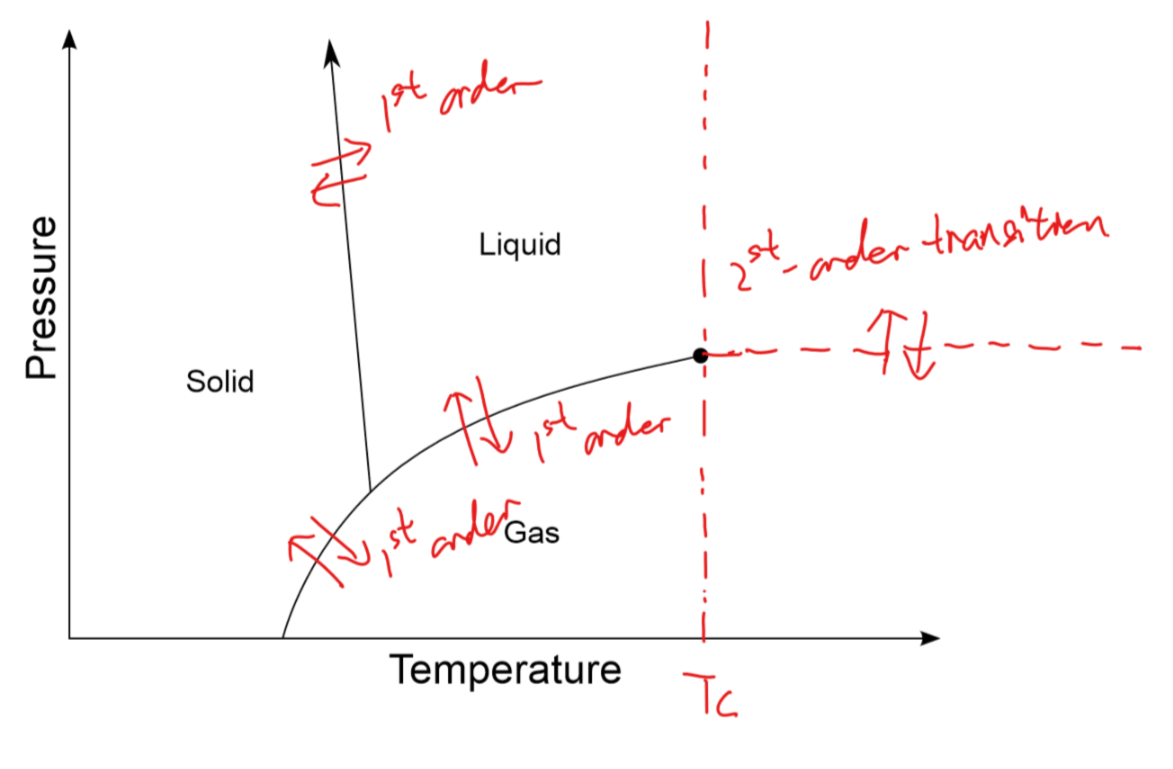
\includegraphics[scale=0.5]{PIC/hw1.png}
	\end{figure}
\end{exer}
\begin{exer}
	By the homogeneous relation
\[
f(t,h)= b^{-d}f(b^{y_t} t, b^{y_h} h)
\]
we have 
\[
f(t,h)= t^{\frac{d}{y_t}}g(\alpha)
\]
where $g(\alpha) = f(1,\alpha)$ and $\alpha = t^{-\frac{y_h}{y_t}}h$. It is easy to see that $\alpha$ is invariance under scaling transformation $x \to x/b$.
Hence we have 
\[
\begin{aligned}
&C(t,0) = -T \frac{\partial ^2 f}{\partial T ^2}\big|_{h=0} = - \frac{1}{T_c} t^{\frac{d}{y_t}-2}g''(0) \\
& M(t,0) = -\frac{\partial f}{\partial B}\big|_{h=0} =t^{\frac{d-y_h}{y_t}}g'(0)\\
& \chi(t,0) = \frac{\partial^2 f}{\partial B^2}\big|_{h=0} = t^{(d-2y_h)/y_t} g''(0)\\
\end{aligned}
\]
As function with single variable $h$, $\lim_{t \to 0}  M(t,h) \sim h^{\frac{1}{\delta}}$, which implies that $g'(\alpha) \sim \alpha^{\frac{1}{\delta}}$ since $\alpha$ is linear function of $h$. Hence we have 
\[
\lim_{t \to 0} M = \lim_{t \to 0} t^{(d-y_n - \frac{y_n}{\delta})}h ^{1/\delta}
\]
since it is non-zero, we have $d- y_n - y_n \frac{1}{\delta}=0$. Hence we have 
\[
\delta = \frac{y_h}{d-y_h}
\]	
\end{exer}
\begin{exer}
	We have following relation
	\begin{equation}\label{eq1}
	G_{\sigma}(\mathbf{r};t,h) = t^{-2x_{\sigma}}G_\sigma (\frac{\mathbf{r}}{b};b^{y_t}t,b^{y_h}h)
	\end{equation}
	Let $h=0, K= b^{y_t}t$,	
	\[
	G_{\sigma}(\mathbf{r};t,0) = t^{2x_{\sigma}/y_{t}}G_\sigma (\frac{\mathbf{r}}{K t^{-1/y_{t}}};K,0)
	\]
	Since $ G_{\sigma}(\mathbf{r}) \sim r^{-\tau} e^{-\frac{r}{\xi}}$, we have $\xi \sim t^{-1/y_t}$. It implies $\nu = 1/y_t$. With relation \ref{eq1}, we have 
	\[
	\chi(t,h)= \frac{1}{T} \int d^d \mathbf{r} G_\sigma (\mathbf{r};t,h)= t^{d-2x_\sigma} \chi (b^{y_t}t, b^{y_h}h)
	\]
	So $\gamma = (d-2x_\sigma)/y_t$. But we have $\eta = 2 x_\sigma +2 -d$ for finite limit of $G(r)$ when $t \to 0$ and $h=0$. Therefore, we get
	\[
	\gamma = \nu(2-\eta)
	\]With scaling relations
	\[
	\begin{aligned}
	\alpha + 2 \beta + \gamma =2\\
	\alpha + \beta (1+\delta) =2\\
	\end{aligned}
	\]
	and $\alpha = 2 -d \nu$, we have
	\[
	\begin{aligned}
	\beta &= \frac{d\nu -2\nu + \nu \eta}{2}\\
	\delta &= \frac{d-\eta +2}{d+\eta -2}\\
	\end{aligned}
	\]
	\end{exer}
\begin{exer}
	By listed commutation relations, we have, for $r, s > 0$,
	\[
	\begin{aligned}
	&[D, J_{rs}]= [D, L_{rs}] = \frac{i}{2} [D, [K_r, P_s]]\\
	 & =-\frac{i}{2}\big([P_s,[D,K_r]]+ [K_r,[P_s,D]]\big)\\
	 & =\frac{1}{2}[P_s, K_r] -\frac{1}{2}[K_r, P_s]\\
	 &=0
	\end{aligned}
	\]
	For $r=-1,s=0$, $[D,J_{rs}]= [D,D]=0$. For $r=-1, s\neq 0$, $[D,J_{-1,s}]=[D,\frac{1}{2}(P_s - K_s)]= \frac{i}{2}(P_s +K_s)$. For $r=0$, $[D, J_{0s}] = \frac{i}{2}(P_s - K_s)$. Hence (2,25) is satisfied when $(m,n)=(-1,0)$.
	
	If $(m,n)=(-1,n)$, then we have 
	\[
	[J_{mn},J_{rs}] = \frac{1}{2}[P_n, J_{rs}] -\frac{1	}{2} [K_n, J_{rs}]
	\]
	With listed commutation relations, we can easily check it coincides with (2,25) respectively. Similarly check in the case of $(m,n)= (0,n)$. 
\end{exer}
\newpage
\section{Homework 2}
\subsection{$SL_2(\mathbb{C})$}
\begin{exer}
	We have $\det X = t^2-(x^2+y^2+z^2)$. Since points in $\mathbb{R}^{1,3}$ can be written with Pauli matrix as base. Elements in $SO(1,3)$ can be viewed as action on $M_2(\mathbb{C})$ with form $P \mapsto PXP^*$, which preserve det of $X$.
	We have exact sequence of groups as follows:
	\[\begin{tikzcd}
		0 \ar[r] &\mathbb{Z}_2 \ar[r] &SL_2(\mathbb{C}) \ar[r,"sp"]&SO(1,3) \ar[r]&1 
	\end{tikzcd}\]
	where $\text{sp}$ is map $P \mapsto (X \mapsto PXP^*)$. Since for $P \in SL_2(\mathbb{C})$, $\det(PXP*) = \det(X) = t^2-(x^2+y^2+z^2)$, $sp$ is well-defined. Hence $SO(1,3) \cong SL_2(\mathbb{C})/\mathbb{Z}_2$.
\end{exer}
\begin{exer}
	\begin{itemize}
		\item \[
		z \mapsto \frac{(z_2 -z_3)(z-z_1)}{(z_2-z_1)(z-z_3)}
		\]
		\item We have
		\[
		\begin{aligned}
		(w_1 -w_3)=&\frac{(az_1+b)(cz_3+d)-(az_2 +b)(cz_4+d)}{(cz_1+d)(cz_3+d)}\\
		=&\frac{z_1-z_3}{(cz_1+d)(cz_3+d)}
		\end{aligned}
		\]
		Hence we have $[z_1,z_2,z_3,z_4]=[w_1,w_2,w_3,w_4]$.
	\end{itemize}
\end{exer}
\subsection{Three-point function}
\begin{exer}
	Let $\langle\phi_1(z_1)\phi_2(z_2)\phi_3(z_3)\rangle =f(z_{12},z_{23},z_{13})$. Under scalar transformation $z_i \mapsto \lambda z_i$, we have
	\[
	f(z_{12},z_{23},z_{13})=\lambda^{h_1+h_2+h_3}f(\lambda z_{12},\lambda z_{23},\lambda z_{13})
	\]
	Therefore, $f$ is with form
	\[
	f(z_{12},z_{23},z_{13})=\frac{C_{123}}{z_{12}^a z_{23}^b z_{13}^c}
	\]
	where $a+b+c = h_1 +h_2 +h_3$.
	Then under comformal transformation $z_i \mapsto \frac{1}{z_i}$, we have
	\[
	{z_1}^{-2h_1}{z_2}^{-2h_2}{z_3}^{-2h_3} \frac{(z_1z_2)^a(z_2 z_3)^b(z_1z_3)^c}{z_{12}^a z_{23}^b z_{13}^c}= \frac{1}{z_{12}^a z_{23}^b z_{13}^c}
	\]
	Hence $a= h_1 +h_2 -h_3, b=h_2 + h_3 -h_1, c= h_1 +h_3 - h_2$.
\end{exer}
\subsection{Energy-momentum tensor}
\begin{exer}
	\begin{itemize}
		\item \[
		T^{\mu \nu} = -\eta^{\mu \nu}\partial_{k}\varphi \partial^{k}\varphi + 2 \partial^{\mu}\varphi \partial^{\nu}\varphi
		\]
		\item We have
		\[
			\delta \sqrt{g}= -\frac{1}{2}\sqrt{g} g_{\mu\nu} \delta g^{\mu\nu}
		\]
		Therefore,
		\[
		\begin{aligned}
		\tilde{T}^{\mu\nu} &=\frac{2}{\sqrt{g}}\frac{\delta S}{\delta g^{\mu\nu}}\\
		&=\frac{1}{2} (-\delta_{\mu\nu}+2) \partial_{\mu} \varphi \partial_{\nu}\varphi
		\end{aligned}
		\]
	\end{itemize}
\end{exer}
\newpage
\section{Homework 4}
\subsection{Derivations}
	\subsubsection{Energy-momentum tensor in complex coordinate}
	Since 
	\[
	\begin{aligned}
	&\partial_0 \Phi = \partial_z \Phi + \partial_{\bar{z}}\Phi\\&\partial_1 \Phi = i\partial_z \Phi - i \partial_{\bar{z}}\Phi
	\end{aligned}
	\]
	we have \[
	\begin{aligned}
	&\partial_z \Phi =\frac{1}{2} \partial_0 \Phi - \frac{i}{2} \partial_1 \Phi\\& \partial_{\bar{z}} \Phi = \frac{1}{2} \partial_0 \Phi+ \frac{i}{2} \partial_1 \Phi
	\end{aligned}
	\] 
	Also, since there are metric tensors in complex coordinates
	\[
	\begin{aligned}
	g^{\alpha \beta}= \begin{pmatrix}
	0&2 \\
	2&0\\
	\end{pmatrix}& &g_{\alpha \beta}\begin{pmatrix}
	0& \frac{1}{2}\\
	\frac{1}{2}& 0\\
	\end{pmatrix}
	\end{aligned}
	\],
	we have $\partial^z \Phi = 2 \partial_{\bar{z}}$ and $\partial^{\bar{z}} \Phi = 2\partial_{\bar{z}} \Phi$. Therefore, from definition of energy-momentum tensor
	\[T_{\alpha \beta}= - g_{\alpha \beta} \mathcal{L}+ \frac{\partial \mathcal{L}}{\partial (\partial^\alpha \Phi)} \partial_\beta \Phi
	\] we get expression of them in complex coordinates
	\[
	\begin{aligned}
	&T_{zz} = \frac{1}{4}\big( \frac{\partial \mathcal{L}}{\partial_0 \Phi} \partial_0 \Phi - i \frac{\partial}{\partial_1 \Phi} \partial_0 \Phi - i \frac{\partial \mathcal{L}}{\partial_0 \Phi} \partial_1 \Phi - \frac{\partial \mathcal{L}}{\partial_1 \Phi} \partial_1 \Phi\big)\\
	&T_{\bar{z}\bar{z}} = \frac{1}{4}\big( \frac{\partial \mathcal{L}}{\partial_0 \Phi} \partial_0 \Phi + i \frac{\partial}{\partial_1 \Phi} \partial_0 \Phi + i \frac{\partial \mathcal{L}}{\partial_0 \Phi} \partial_1 \Phi - \frac{\partial \mathcal{L}}{\partial_1 \Phi} \partial_1 \Phi \big)\\
	&T_{z \bar{z}} = - \frac{1}{2} \mathcal{L} + \frac{1}{4} \big( \frac{\partial \mathcal{L}}{\partial_0 \Phi} \partial_0 \Phi - i \frac{\partial}{\partial_1 \Phi} \partial_0 \Phi + i \frac{\partial \mathcal{L}}{\partial_0 \Phi} \partial_1 \Phi + \frac{\partial \mathcal{L}}{\partial_1 \Phi} \partial_1 \Phi\big)\\
	&T_{z \bar{z}} = - \frac{1}{2} \mathcal{L} + \frac{1}{4} \big( \frac{\partial \mathcal{L}}{\partial_0 \Phi} \partial_0 \Phi + i \frac{\partial}{\partial_1 \Phi} \partial_0 \Phi - i \frac{\partial \mathcal{L}}{\partial_0 \Phi} \partial_1 \Phi + \frac{\partial \mathcal{L}}{\partial_1 \Phi} \partial_1 \Phi\big)\\
	\end{aligned}
	\]
	Hence 
	\[
	\begin{aligned}
	&T_{zz} = \frac{1}{4} (T_{00} - 2i T_{10} - T_{11})\\
	&T_{\bar{z} \bar{z}} = \frac{1}{4} (T_{00} +2i T_{10} - T_{11})\\
	&T_{z\bar{z}} =T_{\bar{z}z}= \frac{1}{4} (T_{00} + T_{11})\\
	\end{aligned}
	\]
\subsubsection{Schwarzian derivative}
\[
\tilde{T}(z+\epsilon(z)) = (1+ \partial_z \epsilon(z))^{-2}\Big[T(z)- \frac{c}{12}\big(\frac{\partial_z^3\epsilon(z)}{1+\partial_z\epsilon(z)}-\frac{2}{3} \frac{\partial_z^2 \epsilon(z)}{1+\partial_z \epsilon(z)}\big)\Big]
\]
Since 
\[
\frac{1}{1+\partial_z \epsilon(z)} = 1- \partial_z \epsilon(z) + (\partial_z \epsilon)^2 + \cdots
\]
we have 
\[
\begin{aligned}
\tilde{T}(z+ \epsilon(z)) &\approx T(z)(1-2\partial_z \epsilon(z)) - \frac{c}{12} (\partial^3_z \epsilon(z) - \frac{2}{3} \partial^2_z \epsilon(z))\\
& \approx T(z) - 2 \partial_z\epsilon(z) T(z) - \frac{c}{12}\partial^3_z\epsilon(z)
\end{aligned}
\]
Hence
\[
\tilde{T}(z+ \epsilon(z)) - \big[\epsilon(z)\partial_z T(z) +T(Z)\big] \approx -\frac{c}{12} \partial^3_z\epsilon(z) - 2 \partial_z\epsilon(z)T(z) -\epsilon(z)\partial_z T(z) 
\]
It implies that $\delta_\epsilon(T(z)) = -\frac{c}{12} \partial^3_z\epsilon(z) - 2 \partial_z\epsilon(z)T(z) -\epsilon(z)\partial_z T(z) $.
\subsubsection{Virasoro algebra}
The Larrent expansion of $z^{n+1}$ around $\omega$ is 
\[
z^{n+1}= (z- \omega)^{n+1} + \binom{n+1}{1} \omega (z-\omega)^n + \cdots + \binom{n+1}{i}\omega^i (z-\omega)^{n+1 -i} +\cdots + \omega^{n+1}
\]
 Hence we have following residues:
 \[
 \begin{aligned}
 &\res_{\omega} \frac{z^{n+1}}{(z-\omega)^4}= 2 \pi i \frac{(n+1)n(n-1)}{6} \omega^{n-2}\\ 
&\res_{\omega} \frac{z^{n+1}}{(z-\omega)^2}= 2 \pi i (n+1) \omega^n\\
&\res_{\omega} \frac{z^{n+1}}{z-\omega}= 2 \pi i \omega^{n+1}
 \end{aligned}
 \]
  Hence we have 
  \[
  \begin{aligned}
  &[L_n, L_m] = \frac{1}{(2 \pi i )^2} \oint_0 d \omega\ \omega^{m+1} \oint_\omega dz\ z^{n+1} \big(\frac{c}{2(z-\omega)^4} + \frac{2T(\omega)}{(z-\omega)^2} + \frac{\partial_\omega T(\omega)}{(z-\omega)} + \text{regular part}\big)\\
  &= \frac{1}{2 \pi i} \oint_0 d\omega\ \omega^{m+1} \big( \frac{c}{12}(n+1)n(n-1) \omega^{n-2} + 2(n+1) \omega ^n T(\omega) + \omega^{n+1} \partial_{\omega} T(\omega) \big)&\\
 &= \frac{1}{2 \pi i} \Big\{\oint_0 d\omega\ \Big( \frac{c(n+1) n(n-1)}{12} \omega^{m+n-1} )\Big) - (m-n) \oint_0 d\omega \omega^{m+n +1 } T(\omega) \Big\}&\\
 &= \frac{c}{12} n (n^2-1) \delta_{n+m,0} - (m-n) L_{n+m}
  \end{aligned}
  \]
 \subsubsection{Commutation relations in free boson}
 We have 
 \[
 \varphi = \varphi_0 + \frac{4\pi}{l} \pi t + i \sum_{n \neq 0} \frac{1}{n} \Big( a_n e^{-2 \pi in (t-x)/l} + \bar{a}_n e^{-2 \pi n (t+x)/l}\Big)
 \]
 on cylinder. 
 \[
 \Pi = \frac{\pi_0}{l}+ \frac{1}{2l} \sum_{n \neq 0} \Big(a_n e^{-2\pi i n (t-x)/l} + \bar{a}_n e^{-2 \pi i n (t+x) /l}\Big)
 \]
  With $[\Pi, \Pi]=0$, we can get $[\pi_0, a_n] =0$ and $[\pi_0, \bar{a}_n]=0$. Furthermore, since $[\varphi, \varphi]=0$, we have $[\varphi_0, a_n]= [\varphi_0 ,\bar{a}_n]=0$.
  \[
  \begin{aligned}
  &i \delta(x-y)=[\varphi(x,t), \Pi(y,t)]&= \frac{1}{l} [\varphi_0, \pi_0] + \frac{i}{2l} \sum_{n \neq 0, m \neq 0} \frac{1}{n}\Big([a_n, \bar{a}_m] \exp(-2 \pi i [(n+m)t -nx+my]/l)\\
  && + [\bar{a}_n, a_m] \exp(-2\pi i [(n+m)t +nx -my]/l) \\
  && + [a_n, a_m] \exp(-2\pi i [(n+m)t -nx -my]/l) \\
  && + [\bar{a}_n, \bar{a}_m] \exp(-2\pi i [(n+m)t +nx+my]/l)\Big)\\
  \end{aligned}
  \]
  Since $t$ can be arbitrary, $[a_n, \bar{a}_m] = [\bar{a}_n, a_m] =0$ when $n+m \neq 0$. Then let $t=0$, we get\[
  \begin{aligned}
  i \delta(x-y)&=[\varphi(x,0), \Pi(y,0)] \\
  &= \frac{1}{l}[\varphi_0, \pi_0] + \frac{i}{2l} \sum_{n \neq 0}\frac{1}{n} \Big([a_n, \bar{a}_{-n}] e^{- 2 \pi i (-nx -ny)/l} + [\bar{a}_n, a_{-n}] e^{-2 \pi i (nx+ny)/l} + \text{other terms}\Big)\\
   & = \frac{1}{l}[\varphi_0, \pi_0] + \frac{i}{l} \sum_{n \neq 0} \Big( \frac{2[a_n, \bar{a}_{-n}]}{n}  \Big)e^{2 \pi i(n(x+y))/l} + \text{other terms}
  \end{aligned}
  \]
  Since $e^{2 \pi i (n(x+y))/l}$ is independent of $x-y$, then its coefficient is zero. Hence $[a_n, \bar{a}_{-n}]=0$.
  Take integral of both left and right side, we can get $[\varphi_0, \pi_0] = i$ and $[a_n, a_{-n}] = [\bar{a}_n, \bar{a}_{-n}] = 1$.
 \subsubsection{Action of free fermion}
 \[
 S = \frac{1}{4\pi} \int d^2 x \psi^\dagger \gamma^0(\gamma^0 \partial_0 \psi + \gamma^1 \partial_1 \psi)
 \]
 But
 \[
 \gamma^0(\gamma^0 + \gamma^1) \psi = \begin{pmatrix}
 \partial_0 + i \partial_1& 0 \\
 0 & \partial_0 - i \partial_1\\
 \end{pmatrix} \psi
 \]
 Write $\psi$ as $\begin{pmatrix}
 \varphi\\ \bar{\varphi}
 \end{pmatrix}$, then we have $$ \gamma^0(\gamma^0 + \gamma^1) \psi = \begin{pmatrix}
 2\partial_{\bar{z}} \varphi\\ 2 \partial_{z} \bar{\varphi}
 \end{pmatrix}$$
 Hence 
 \[
	S = \frac{1}{2\pi} \int d^2 x (\bar{\varphi} \partial_{z} \bar{\varphi} +  \varphi \partial_{\bar{z}} \varphi)
 \]
 \subsubsection{$TT$ OPE in free fermion}
By derivative, we get 
\[
\begin{aligned}
\langle \psi (z), \partial_\omega \psi(\omega) \rangle \sim \frac{1}{(z-\omega)^2}& \\
 \langle \partial_z \psi , \partial_\omega \psi \rangle \sim \frac{-2}{(z-\omega)^3}&\\
\end{aligned}
\]
Hence 
\[
\begin{aligned}
T(z) \partial_\omega \psi(\omega) & = \frac{1}{2} : \psi(z) \partial_z \psi(z): \partial_\omega \psi(\omega)\\
& \sim -\frac{\psi(\omega)}{(z-\omega)^3} - \frac{1}{2} \frac{\partial_\omega \psi (\omega)}{(z-\omega)^2}
\end{aligned}
\]
and 
\[
\begin{aligned}
T(z)T(\omega) &= \frac{1}{4} : \psi(z) \partial_z \psi(z) :: \psi(\omega) \partial_\omega \psi(\omega)\\
& \sim \frac{1}{4} \big\{ - \frac{:\partial_z \psi(z) \partial_\omega \psi(\omega)}{z-\omega} + \frac{2: \psi(z) \psi(\omega):}{(z-\omega)^3} - \frac{: \psi(z) \partial_\omega \psi(\omega) + \partial_z \psi(z) \psi(\omega):}{(z-\omega)^2} + \frac{1}{(z-\omega)^4} \big\}\\
&\sim \frac{1}{4} \big\{\frac{2 \partial_\omega T(\omega)}{z-\omega} + \frac{4T(\omega)}{(z-\omega)^2} + \frac{1}{(z-\omega)^4}  \big\}
\end{aligned}
\]
\subsection{Vertex operator and OPE}
If we write $\varphi(z,\bar{z})$ into laurent series since $\varphi$ is free boson, then we can find $\exp(ik \varphi)$ is product of infinite exponential components which are commutative. Hence the normal ordering has taylor expansion form
\[
:\exp(ik \varphi(z,\bar{z})): = \sum_{n=0}^{\infty} \frac{(ik)^n}{n!}: \varphi(z,\bar{z})^n:
\]
To justify that $:\exp(ik \varphi):$ is primary field, we calculate its OPE
\[
\begin{aligned}
T(z):\exp{ik \varphi(\omega,\bar{\omega})}:& = - \frac{1}{2} \sum_{n=0}^{\infty} : \partial \varphi(z) \partial \varphi(z) :: \varphi(\omega, \bar{\omega})^n\\
&\sim - \sum_{n=1}^{\infty} \frac{(ik)^n}{n!} n : \partial \varphi(z) \overbrace{\partial \varphi(z) \varphi(\omega,\bar{\omega})} \varphi(\omega,\bar{\omega})^{n-1}:\\
&- \frac{1}{2}\sum_{n=2}^{\infty} \frac{(ik)^n}{n!} n(n-1) : \overbrace{\partial \varphi(z) \overbrace{\partial \varphi(z) \varphi(\omega, \bar{\omega})} \varphi(\omega,\bar{\omega})} \varphi(\omega,\bar{\omega})^{n-2}:\\
&\sim \frac{ik \partial_\omega \varphi(\omega)}{z-\omega}:\exp(ik\varphi): +\frac{k^2}{2(z-\omega)^2} :\exp(ik\varphi):\\
\end{aligned}
\]
This form implies that $:\exp(ik\varphi):$ is primary field with conformal dimension $\frac{k^2}{2}$.
\subsection{$bc$ ghost system}
 \[
 \begin{aligned}
 T(z) b(\omega) & = (-2: b(z) \partial c(z): + :c(z) \partial b(z):) b(\omega)\\
 & 2 \frac{b(z)}{(z-\omega)^2} - \frac{\partial_z b(z)}{z-\omega}\\
 \end{aligned}
 \]
 Take Taylor expansion of $b(z)$ and $\partial_z b(z)$ around $\omega$, we have
 \[
 T(z)b(w) \sim 2\frac{b(\omega)}{(z-\omega)^2} + \frac{\partial_\omega b(\omega)}{z-\omega}
 \]
 Hence the conformal dimension of $b$ is $2$.
 
 Similarly, we have
 \[
 \begin{aligned}
 T(z) c(\omega) & = (-2: b(z) \partial c(z): + :c(z) \partial b(z):) c(\omega)\\
 & \sim - \frac{c(z)}{(z-\omega)^2} + 2\frac{\partial_z c(z)}{z-\omega}\\
 & \sim -\frac{c(\omega)}{(z-\omega)^2} + \frac{\partial_\omega c(\omega)}{z-\omega}
 \end{aligned}
 \]
Hence conformal dimension of $c$ is $-1$.
 \[
 \begin{aligned}
 T(z)T(\omega)&= 4 :b(z) \partial c(\omega): : b(\omega) \partial c(\omega):\\
 & - 2: c(z) \partial b(z) :: b(\omega) \partial c(\omega): - 2: b(z) \partial c(z):: c(\omega) \partial b(\omega):\\
 & + c(z)\partial b(z) :: c(\omega) \partial b(\omega):\\
 \end{aligned}
 \]
 We will calculate it term by term
 \[
 \begin{aligned}
& 4:b(z) \partial c(z):: b(\omega) \partial c(\omega):\\
&\sim 4 \Big(: \overbrace{b(z) \partial c(z)b(\omega) \partial c(\omega)}: + b(z)  \overbrace{\partial c(z)  b(\omega)} \partial c(\omega)+: \overbrace{b(z) \overbrace{\partial c(z) b(\omega)} \partial c(\omega)}: \Big)\\
& \sim \frac{4(-: \partial_z c(z) b(\omega): +: b(z) \partial_\omega c(\omega):)}{(z-\omega)^2} - \frac{4}{(z-\omega)^4}\\
& \sim - \frac{4}{(z-\omega)^4}+\frac{8b(\omega) \partial_\omega c(\omega)}{(z-\omega)^2} + \frac{-4: \partial^2_\omega c(\omega) b(\omega): + 4 \partial_\omega b(z) \partial_\omega c(\omega)}{z-\omega}
 \end{aligned}
 \]
 and
 \[
\begin{aligned}
 &2: c(z) \partial b(z) :: b(\omega) \partial c(\omega):\\
 &
 \sim 2\Big( -: \overbrace{c(z) \partial b(z) b(\omega)} \partial c(\omega) - :c(z)\overbrace{\partial b(z) b(\omega) \partial c(\omega))} - :\overbrace{\partial b(z) \overbrace{c(z) b(\omega)} \partial c(\omega)} \Big)\\
 & \sim  \frac{4}{(z-\omega)^4} + \frac{4: c(z) b(\omega):}{(z-\omega)^3} - \frac{2: \partial b(z) \partial c(\omega)}{(z-\omega)} \\
 & \sim \frac{4}{(z-\omega)^4} + \frac{4:c(\omega) b(\omega):}{(z-\omega)^3} + \frac{4 :\partial_\omega c(\omega) b(\omega):}{(z-\omega)^2} + \frac{2: \partial_\omega^2 c(\omega) b(\omega): -2 : \partial_\omega b(\omega) \partial_\omega c(\omega):}{z-\omega}
\end{aligned}
 \]
 and symmetrically 
 \[
	\begin{aligned}
	&2: b(z) \partial c(z):: c(\omega) \partial b(\omega)\\
	& \sim \frac{4}{(z-\omega)^4} + \frac{4:b(\omega) c(\omega):}{(z-\omega)^3} + \frac{4 :\partial_\omega b(\omega) c(\omega):}{(z-\omega)^2} + \frac{2: \partial_\omega^2 b(\omega) c(\omega): -2 : \partial_\omega c(\omega) \partial_\omega b(\omega):}{z-\omega} 
	\end{aligned}
 \]
 and
 \[
	\begin{aligned}
	&c(z)\partial b(z) :: c(\omega) \partial b(\omega):\\
	& \sim \frac{2: c(\omega) \partial_{\omega}b(\omega) }{(z-\omega)^2} + \frac{-\partial^2_\omega b(\omega) c(\omega)+\partial_\omega c(\omega)\partial_\omega b(\omega)}{z-\omega} - \frac{1}{(z-\omega)^4}
	\end{aligned}
 \]
 Hence we have 
 \[
 T(z)T(\omega) \sim -\frac{13}{(z-\omega)^4} + \frac{2T(\omega)}{(z-\omega)^2} + \frac{\partial T(\omega)}{z-\omega}
 \]
 So the central charge is equal to $-26$.
\subsection{Schwarzian derivatives}
Let $\omega = \frac{az+b}{cz +d}$, then
\[
\begin{aligned}
&\frac{d\omega}{d z} = \frac{ad-bc}{(cz+d)^2}\\
&\frac{d^2\omega}{dz^2} = \frac{-2c(ad-bc)}{(cz+d)^3}\\
&\frac{d^3\omega}{dz^3} = \frac{6c^2(ad-bc)}{(cz+d)^4}\\
\end{aligned}
\]
Hence
\[
\begin{aligned}
\{\omega,z\} & = \frac{6c^2}{(cz+d)^2} -\frac{3}{2}(\frac{-2c}{cz+d})^2\\
&=0\\
\end{aligned}
\]
Then
\[
\begin{aligned}
\Big(\frac{a \omega +b}{c \omega +d}\Big)'_z &= \frac{ad-bc}{(c\omega +d)^2} \omega'_z\\
\Big(\frac{a \omega +b}{c \omega +d}\Big)''_z&= \frac{-2c(ad-bc)}{(c\omega+d)^3}(\omega'_z)^2 + \frac{ad-bc}{(c\omega +d)^2} \omega''_z\\
\Big(\frac{a \omega +b}{c \omega +d}\Big)'''_z&= \frac{6c^2(ad-bc)}{(c\omega +d)^4}(\omega'_z)^3 +3 \frac{-2c(ad-bc)}{(c\omega+d)^3} \omega''_z \omega'_z + \frac{ad-bc}{(c\omega +d)^2} \omega'''_z
\end{aligned}
\]
Hence we have
\[
\{ \frac{a \omega +b}{c\omega+d}, z\} = \frac{6c^2}{(c\omega +d)^2}(\omega'_z)^2 + 3 \frac{-2c}{c\omega+d} \omega''_z + \frac{\omega'''_z}{\omega'_z} - \frac{3}{2}\Big(\frac{-2c}{c\omega +d} \omega'_z + \frac{\omega_z''}{\omega'_z}\Big)^2
\]
It is equal to $\{\omega, z\}$.
\newpage
\noindent
{\LARGE\underline{\textbf{2d CFT}}}\\
{\hfill\large  \underline{\textbf{邹海涛}} \\
	\hfill ID: 17210180015}\\
\section{Modular invariant}
\[
Z_R(z, \bar{z}) = \frac{1}{\lvert \eta (\tau) \rvert ^2} \sum_{m,n} q^{\frac{1}{2}(\frac{m}{R}+ \frac{Rn}{2})^2} \bar{q}^{\frac{1}{2} (\frac{m}{R} - \frac{Rn}{2})^2}
\]
First, we compute the sum part. Let $z= x+ iy$
\[
\begin{aligned}
\sum_{m,n}&= \sum_{m.n}q^{\frac{1}{2} ( \frac{m}{R}+ \frac{Rn}{2})^2} \bar{q}^{\frac{1}{2}(\frac{m}{R}+ \frac{Rn}{2})^2}\\
&= \sum_{m,n}\exp\big\{z \pi i (\frac{m}{R}+ \frac{Rn}{2})^2 -\bar{z} \pi i (\frac{m}{R}- \frac{Rn}{2})^2 \big\}\\
&= \sum_{m.n} \exp\big\{-\frac{2\pi y}{R^2}m^2 - \frac{\pi y R^2}{2}n^2 + 2\pi i xmn \big\}\\
&= \sum_{m,n} \exp\big\{- \frac{2\pi y}{R^2} (m - \frac{R^2x i}{2y}n )^2\big\} \exp \big\{-\frac{\pi R^2 x^2 }{2y} n^2 - \frac{\pi R^2 y}{2}n^2\big\}
\end{aligned}
\]
Let $ a= \frac{R^2}{2y}, b = \frac{\pi R^2 x}{y}n$ in Possion formula, then we have 
\[
\begin{aligned}
&= \frac{R}{\sqrt{2y}} \sum_{m,n}\exp \big\{-\frac{\pi R^2}{2y} m^2 + \frac{\pi R^2 x}{y}mn - \frac{\pi R^2 x^2}{2y}n^2 -\frac{\pi R^2}{2} n^2\big\}\\
&= \frac{R}{\sqrt{2y}}\sum_{m,n} \exp\big\{- \frac{\pi R}{2y}( m^2 - xmn + (xn)^2+(yn)^2\big\}\\
& = \frac{R}{\sqrt{2y}} \sum_{m,n}\exp\big\{- \frac{\pi R}{2y}( (m-xn)^2+ (yn)^2)\big\}\\
& = \frac{R}{\sqrt{2y}} \sum_{m,n}\exp\big\{- \frac{\pi R}{2y}\lvert n z -m \rvert ^2\big\}\\
\end{aligned}
\]
Hence when $z \mapsto -1/z$, the sum part becomes
\[
\frac{R\lvert z\rvert}{\sqrt{2y}} \sum_{m,n}\exp\big\{- \frac{\pi R}{2y}\lvert n \bar{z} -m \rvert ^2\big\}= \frac{R\lvert z\rvert}{\sqrt{2y}} \sum_{m,n}\exp\big\{- \frac{\pi R}{2y}\lvert n z -m \rvert ^2\big\}
\]
Since we have
\[
\eta(- \frac{1}{z})= \sqrt{-iz} \eta(z)
\]
it norm is 
\[
\lvert \eta(- \frac{1}{z}) \rvert = \sqrt{\lvert z \rvert} \lvert \eta(z) \rvert
\]
Hence we can conclude that
\[
Z_R(z, \bar{z}) =Z_R(- \frac{1}{z}, -\frac{1}{\bar{z}})
\]
\section{Modular transformation}
We have 
\[
\begin{aligned}
\gamma \cdot \tau &= \frac{a\tau + b}{c\tau + d}\\
& = \frac{(a\tau +b)(c \bar{\tau} +d)}{\lvert c \tau +d \rvert^2}\\
& = \frac{ac \lvert \tau \rvert^2 + bc \bar{\tau} + ad \tau}{\lvert c\tau + d\rvert ^2}\\
& = \frac{ac \lvert \tau \rvert ^2 + (ad+ bc)\re \tau+ i(ad-bc) \im \tau}{\lvert c\tau +d \rvert ^2}\\
\end{aligned}
\]
Since $ad-bc=1$, we can conclude that \[\im(\gamma \cdot \tau) = \frac{\im \tau}{\lvert c\tau +d\rvert^2}\]
In the upper-half plane, the gray region can be described as
\[
\begin{aligned}
-\frac{1}{2} \leq \re \tau \leq \frac{1}{2}\\
\lvert \tau \rvert > 1
\end{aligned}
\]
If $S$ acts on the gray region, then we have $S(z) = -\frac{1}{z} = - \frac{\bar{z}}{\lvert z \rvert ^2}$, hence it sends the region to the red region. And the blue region is the image of the gray origin under $T$. Finally, the transformation $ST$, maps to the green region.
\section{Boson-Fermion correspondence}
\subsection{$:e^{i\varphi}: \cong \psi$, $:e^{-i\varphi} \cong \bar{\psi}$}
Calculate the OPE of $:e^{i \varphi}:$ directly
\[
\begin{aligned}
:e^{i\varphi(z)}::e^{i\varphi(0)} &\sim\sum_{m,n,k} \frac{k!}{m!n!}\binom{m}{k}\binom{n}{k} (-\wick{\c\varphi(z)\c\varphi(0)}):(i\varphi(0)^{m+n-k}):\\
& \sim \sum_{m,n,k} \frac{1}{k!}\ln^k(z) \frac{1}{(m-k)!}\frac{1}{(n-k)!}:i\varphi(0)^{m+n-k}:\\
&= e^{\ln z} : e^{2i\varphi(0)}:\\
&\sim 0
\end{aligned}
\]
The OPE of $T_\varphi$ with vertex operators $:e^{i\varphi}$ and $:e^{-i\varphi}$ is given in last homework
\[
T_\varphi (z) :e^{i \varphi}: \sim \frac{\partial_z \exp(i\varphi)(0)}{z} +\frac{\exp(i\varphi)(0)}{2z^2}
\]
\[
T_\varphi (z) :e^{-i \varphi}: \sim \frac{\partial_z \exp(-i\varphi)(0)}{z} +\frac{\exp(-i\varphi)(0)}{2z^2}
\]
On the other hand, the OPE of $T_\psi$ with $\psi$ and $\bar\psi$ can be calculated as follows.
First,
\[
\begin{aligned}
\partial\bar{\psi}(z) \psi(0) &\sim \frac{1}{2}(\partial\psi^1(z) - i \partial\psi^2(z))(\psi^1(0)+ i \psi^2(0))\\
& \sim - \frac{1}{z^2}
\end{aligned}
\]
\[
\begin{aligned}
\bar{\psi}(z) \partial\psi(0) &\sim \frac{1}{2}(\psi^1(z) - i \psi^2(z))(\partial\psi^1(0)+ i \partial\psi^2(0))\\
& \sim \frac{1}{z^2}
\end{aligned}
\]
and
\[
\begin{aligned}
 \bar{\psi}(z)\psi(0) & \sim \frac{1}{2} (\psi^1(z) - i\psi^2(z) )(\psi^1(0)+ i\psi(0))\\
 & \sim \frac{1}{z}
\end{aligned}
\]
Hence
\[
\begin{aligned}
T_\varphi(z) \psi(0) =& - \frac{1}{2}\wick{:\psi  \c2{\partial\bar{\psi}}:\c2\psi(0) - \frac{1}{2}: \c2{\bar{\psi}} \partial \psi: \c2 \psi(0)}\\
&\sim - \frac{1}{2}\psi(z)(-\frac{1}{z^2}) + \frac{1}{2} \frac{1}{z} \partial_z\psi(z)\\
&\sim \frac{\psi(0)+ z\partial_z \psi(0)}{2 z^2} + \frac{\partial_z \psi(0)}{2z}\\
&\sim \frac{\psi(0)}{2z^2} + \frac{\partial_z \psi(0)}{z}
\end{aligned}
\]

and
\[
\begin{aligned}
T_\varphi(z) \bar{\psi}(0) =& - \frac{1}{2}\wick{:\c\psi \partial\bar{\psi}:\c{\bar\psi(0)} - \frac{1}{2}: \bar{\psi} \c{\partial \psi}: \c{\bar{\psi}(0)}}\\
&\sim  \frac{1}{2}\partial\bar{\psi}(z)(\frac{1}{z}) - \frac{1}{2} \bar{\psi}(z) (-\frac{1}{z^2})\\
&\sim \frac{\bar{\psi}(0)+ z\partial_z \bar{\psi}(0)}{2 z^2} + \frac{\partial_z \bar{\psi}(0)}{2z}\\
&\sim \frac{\bar{\psi}(0)}{2z^2} + \frac{\partial_z \bar{\psi}(0)}{z}\\
\end{aligned}
\]
\subsection{$i\partial\varphi\cong\psi \bar{\psi}$ }
Also, as calculated before, the OPE of $i\partial\varphi$ is as follows
\[
\begin{aligned}
T_\varphi(z) (i\partial\varphi(0))& \sim \frac{i\partial \varphi(0)}{z^2} + \frac{i \partial^2_z \varphi(0)}{z} 
\end{aligned}
\]
\[
\begin{aligned}
T_\psi(z) \psi \bar{\psi}(0)&= -\frac{1}{2} : \psi(z) \partial\bar{\psi}(z): \psi(0) \bar{\psi}(0) - \frac{1}{2}: \bar{\psi}(z) \partial \psi(z) : \psi(0) \bar{\psi}(0)\\
&\sim \wick{-\frac{1}{2} : \psi(z) \c{\partial \bar{\psi}(z)}\c{\psi(0)} \bar{\psi}(0):} - \frac{1}{2}: \wick{\c{\psi}(z) \partial \bar{\psi}(z) \psi(0) \c{\bar{\psi}(0)}}:\\
& \wick{-\frac{1}{2}: \c2{\psi}\c1{\partial \bar{\psi}} \c1{\psi(0)} \c2{\bar{\psi(0)}}:}\\
& \wick{-\frac{1}{2}:\c1{\bar{\psi}(z)} \partial\psi(z) \c1\psi(0) \bar{\psi}(0:) - \frac{1}{2}: \bar{\psi}(z) \c1{\partial\psi(z)} \psi(0) \c1{\bar{\psi}(0)} } \\
& \wick{-\frac{1}{2}: \c2{\bar{\psi}(z)} \c1{\partial\psi(z)} \c2{\psi(0)} \c1{\bar{\psi}(0)}}\\
&\sim  \frac{\partial \bar{\psi}(0) \psi(0)- \partial \psi(0) \psi(0) + \partial\psi(0) \bar{\psi}(0) - \partial\bar{\psi}(0)\psi(0)}{2z}\\&+\frac{\bar{\psi}(0) \psi(0)  - \psi(0) \bar{\psi}(0)}{2z^2}\\
&\sim \frac{\partial(\psi\bar{\psi})(0)}{z}+ \frac{\psi\bar{\psi}(0)}{z^2}
\end{aligned}
\]
(Tips: I'm confused here. Is the $i$ in $i \partial\varphi$ necessary? I failed to get it in Fermion side.)
\subsection{$T_\varphi \cong T_\psi$}
Finally, we compute the TT OPE for $\varphi$ and $\psi$. We have
\[
T_\varphi(z) T_\varphi(0) \sim \frac{1/2}{z^4} + \frac{2T_\varphi(0)}{z^2} + \frac{\partial T_\varphi(0)}{z}
\]
In complex Fermion case, we have
\[
\begin{aligned}
T_\psi(z) T_\psi(0) &\sim \frac{1}{4} \Big[: \psi(z) \partial \bar{\psi} (z):: \psi(0) \partial\bar{\psi}(0): + : \bar{\psi}\partial \psi(z):: \psi(0) \partial\bar{\psi}(0):\\
& + :\psi(z)\partial\bar{\psi}(z):: \bar{\psi}(0) \partial\bar{\psi}(0): + : \bar{\psi}(z)\partial\psi(z)::\bar{\psi}(0) \partial\psi(0):\Big]\\
& \sim \frac{1}{4}\Big[\wick{:\c{\psi(z)} \partial\bar{\psi}(z)\psi(0)\c{\partial\bar{\psi}(0)}+: \psi(z)\c{\partial\bar{\psi}(z)} \c{\psi(0)} \partial\bar{\psi}(0): + : \c1{\psi(z)}\c2{\partial\bar{\psi}(z)} \c2{\psi(0)} \c1{\partial\bar{\psi}(0)} } \Big]\\
&+\frac{1}{4}\Big[\wick{:\c{\bar\psi(z)} \partial\psi(z)\c{\psi(0)}\partial\bar{\psi}(0)+: \bar{\psi(z)}\c{\partial\psi(z)} \psi(0) \c{\partial\bar{\psi}(0)}: + : \c1{\bar{\psi(z)}}\c2{\partial\psi(z)} \c1{\psi(0)} \c2{\partial\bar{\psi}(0)} } \Big]\\
&+\frac{1}{4}\Big[\wick{:\c{\psi(z)} \partial\bar{\psi(z)}\c{\bar\psi(0)}\partial\psi(0)+: \psi(z)\c{\partial\bar\psi(z)} \bar{\psi(0)} \c{\partial\psi(0)}: + : \c1{\psi(z)}\c2{\partial\bar\psi(z)} \c1{\bar\psi(0)} \c2{\partial\psi(0)} } \Big]\\
&+\frac{1}{4}\Big[\wick{:\c{\bar{\psi(z)}} \partial\psi(z)\bar{\psi(0)}\c{\partial\psi(0)}+: \bar{\psi(z)}\c{\partial\psi(z)} \c{\bar\psi(0)} \partial\psi(0): + : \c1{\bar\psi(z)}\c2{\partial\psi(z)} \c2{\bar\psi(0)} \c1{\partial\psi(0)} } \Big]\\
&\sim \frac{1/2}{z^4} + \frac{2T_\psi(0)}{z^2}+ \frac{\partial T_\psi(0)}{z}
\end{aligned}
\]

% !TEX root=../main.tex
\section{Null states at level 3}
\section{Minimal models}
The formula (5.40) implies for minimal model $\mathcal{M}_{2,2n+1}$, the central charge is 
\[
\begin{aligned}
c & = 1 - 6 \frac{(2-2n-1)^2}{2(2n+1)}\\
& =  - \frac{2(6n-1)(n-1)}{2n+1}
\end{aligned}
\]
And in this model, the formulas (5.44) and (5.45) becomes
\[
k_{\text{max}} = \begin{cases}
m+r -1 & \text{ if } m+r \leq 2n+2\\
2(2n+1) -(m+r-1) & \text{ if } m+r > 2n+2\\
\end{cases}
\]
and 
\[
l_{\text{max}} = \begin{cases}
3-(s+n) & \text{ if } s+n \geq 2\\
s+n-1& \text{ if } s+n = 1 \\
\end{cases}
\]
Hence we get $(s,n)= (1,1)$ since $l_{\text{max}} \geq 1$. And we also have $2 \leq m+r \leq 6$. So $(m,r)$ has following possibilities
\[
\begin{aligned}
k_{\text{max}}= 1:\ &(1,1) & &\\
k_{\text{max}}= 2:\ &(1,2) & &\\
k_{\text{max}}= 3:\ &(1,3) &(2,2)&\\
k_{\text{max}}= 2:\ &(1,4) & (2,3)&\\
k_{\text{max}}= 1:\ &(1,5) & (2,4) &\ (3,3)\\
\end{aligned}
\]
So we have fusion rules
\[
\begin{aligned}
 &\phi_{(1,1)} \times \phi_{(1,1)} = \phi_{(1,1)}\\
 & \phi_{(1,1)} \times \phi_{(2,1)} = \phi_{(2,1)}\\
 & \phi_{(2,1)} \times \phi_{(2,1)} = \phi_{(1,1)} + \phi_{(3,1)}\\
 & \phi_{(1,1)} \times \phi_{(3,1)} = \phi_{(3,1)}\\
 & \phi_{(1,1)} \times \phi_{(4,1)} = \phi_{(4,1)} \\
 & \phi_{(2,1)} \times \phi_{(3,1)} = \phi_{(2,1)} \\
 & \phi_{(1,1)} \times \phi_{(5,1)} = \phi_{(5,1)} \\
 & \phi_{(2,1)} \times \phi_{(4,1)} = \
\end{aligned}
\]
\newpage
\section{Week 8}
\subsection{Derivation}
We have following equations
\begin{eqnarray}
	\partial_z F(z\bar{z}) = \bar{z}F'(z\bar{z})\\
	\partial_{\bar{z}} F(z\bar{z})= zF'(z\bar{z})
\end{eqnarray}
Combining the definition of $\dot{F}$, we have
\begin{equation}
	\dot{F} = z \partial_z F(z\bar{z}) = \bar{z} \partial_{\bar{z}} F(z\bar{z})
\end{equation}
Since $F(z\bar{z})= z^4 \langle T(z,\bar{z}) T(0,0) \rangle$, we have 
\begin{equation}
	\dot{F} = \bar{z} \partial_{\bar{z}} \big(z^4 \langle T(z,\bar{z}) T(0,0)\rangle \big) = z^4\bar{z} \langle \partial_{\bar{z}}T(z,\bar{z})T(0,0) \rangle
\end{equation}
Similarly, for $G$, we have
\begin{equation}
	\begin{split}
	\frac{1}{4} \dot{G} &= \frac{1}{4}\big(z \partial_z G(z\bar{z})\big)\\
	&=\frac{1}{4} \big(z\partial_z (z^3\bar{z}\langle \Theta(z,\bar{z})T(0,0) \rangle ) \big)\\
	&= \frac{3}{4} z^3 \bar{z}\langle \Theta(z,\bar{z}) T(0,0) \rangle + \frac{1}{4} z^4 \bar{z} \langle \partial_z \Theta(z,\bar{z}) T(0,0) \rangle \\
	&= \frac{3}{4}G - z^4 \bar{z} \langle \partial_{\bar{z}} T(z,\bar{z})T(0,0) \rangle \\
	&= \frac{3}{4} G -\dot{F}
	\end{split}
\end{equation}
With the relation $\frac{1}{4} \langle\partial_z \Theta(z,\bar{z}) T(0,0) \rangle = \langle T(z,\bar{z}) T(0,0) \rangle$, we get
\begin{equation}
\frac{1}{4} \dot{G} = \frac{3}{4} G -\dot{F}
\end{equation}
It implies $\dot{F} + \frac{1}{4} \dot{G} - \frac{3}{4} G=0$. Furthermore, we have
\begin{equation}
\label{eq10}
	\begin{split}
	\dot{G} & = \bar{z} \partial_{\bar{z}} \big(z^3 \bar{z} \langle T(z,\bar{z}) \Theta(0,0) \rangle \big)\\
	& = z^3 \bar{z} \langle T(z,\bar{z}) \Theta(0,0) \rangle + z^3 \bar{z}^2 \langle \partial_{\bar{z}} T(z,\bar{z}) \Theta(0,0) \rangle \\
	&= G - \frac{1}{4} z^3 \bar{z}^2 \langle \partial_z \Theta(z,\bar{z})\Theta(0,0)\rangle
	\end{split}
\end{equation}
and for $H$, we have
\begin{equation}
\label{eq11}
	\begin{split}
	\dot{H} & = z \partial_z \big( z^2 \bar{z}^2 \langle \Theta(z,\bar{z}) \Theta(0,0) \rangle \big)\\
	& =z \big(2 z \bar{z}^2 \langle \Theta (z,\bar{z}) \Theta(0,0) \rangle + z^2 \bar{z}^2 \langle \partial_z \Theta(z,\bar{z}) \Theta(0,0) \rangle \big)\\
	& = 2H + z^3 \bar{z}^2 \langle \partial_z \Theta(z,\bar{z}) \Theta(0,0)\rangle 
	\end{split}
\end{equation}
Combining equation \ref{eq10} and \ref{eq11}, we get 
\[
\dot{G} - G + \frac{1}{4} \dot{H} - \frac{1}{2} H =0
\]
\subsection{\beta-functions}
To compute the integral 
\[
\int_{a < |x_{12}| < a(1+\delta \lambda)} \langle \mathcal{O}(x_1) \mathcal{O}(x_2) \rangle \frac{d x_1}{a^{2-h}} \frac{d x_2}{a^{2-h}}
\]
With OPE $\mathcal{O}(x_1)$ and $\mathcal{O}(x_2)$, we have 
\begin{equation}
	\langle \mathcal{O}(x_1) \mathcal{O}(x_2) \rangle = \frac{C}{|x_{12}|^h} \langle\mathcal{O}(x_2)\rangle
\end{equation} 
Hence we have
\begin{equation}
\label{eq13}
	\begin{split}
	\int_{a < |x_{12} | < a(1+\delta\lambda)} \langle \mathcal{O}(x_1) \mathcal{O}(x_2) \rangle \frac{d x_1}{a^{2-h}} \frac{d x_2}{a^{2-h}} &= \int_{a < |x_{12} | < a(1+\delta\lambda)} \frac{C}{|x_{12}|^h} \frac{dx_1}{a^{2-h}} \langle \mathcal{O}(x_2) \rangle  \frac{dx_2}{a^{2-h}}\\
	&
	\end{split}
\end{equation}
Since $|x_{12}| \sim a$ as $\delta$ infinitesimal, \ref{eq13} becomes 
\begin{equation}
	\begin{split}
	\int_{a < |x_{12} | < a(1+\delta\lambda)} \langle \mathcal{O}(x_1) \mathcal{O}(x_2) \rangle \frac{d x_1}{a^{2-h}} \frac{d x_2}{a^{2-h}} & = a^{-2}C \int_{a < |x_{12} | < a(1+\delta\lambda)} dx_1 \int \langle \mathcal{O}(x) \rangle \frac{dx}{a^{2-h}}\\
	\end{split}
\end{equation}
Since the area of $a < |x_{12} | < a(1+\delta\lambda $ is $\delta \lambda \pi a^2 (\delta \lambda +2)$, we have
\begin{equation}
	\begin{split}
	\int_{a < |x_{12} | < a(1+\delta\lambda)} \langle \mathcal{O}(x_1) \mathcal{O}(x_2) \rangle \frac{d x_1}{a^{2-h}} \frac{d x_2}{a^{2-h}} & = C \delta \lambda \pi (\delta\lambda +2) \int \langle \mathcal{O}(x)\rangle \frac{dx}{a^{2-h}}\\
	& \sim 2 \delta \lambda \pi C \int \langle \mathcal{O}(x) \rangle \frac{dx}{a^{2-h}}
	\end{split}
\end{equation}
Hence the second term is 
\[
\delta \lambda \pi C \hat{g}^2  \int \langle \mathcal{O}(x) \rangle \frac{dx}{a^{2-h}}
\]
Therefore, we get deformation
\begin{equation}
	\text{Def}_{\hat{g}}(\lambda) = \hat{g} + \delta(2-h) \lambda \hat{g} - \delta \pi C \lambda \hat{g}^2 + O(\hat{g}^3)(\lambda)
\end{equation}
Now we have 
\begin{equation}
	\frac{d \hat{g}}{d\lambda} = (2-h) \hat{g} - \pi C \hat{g}^2 + O(\hat{g}^3)
\end{equation}
The $\beta$-function is 
\[
\beta(\hat{g}) = (2-h) \hat{g} - \pi C \hat{g}^2 + O(\hat{g}^3)
\]
Hence near $\hat{g}=0$, we have the picture of curve of $\beta$-function
\begin{figure}[h]
	\centering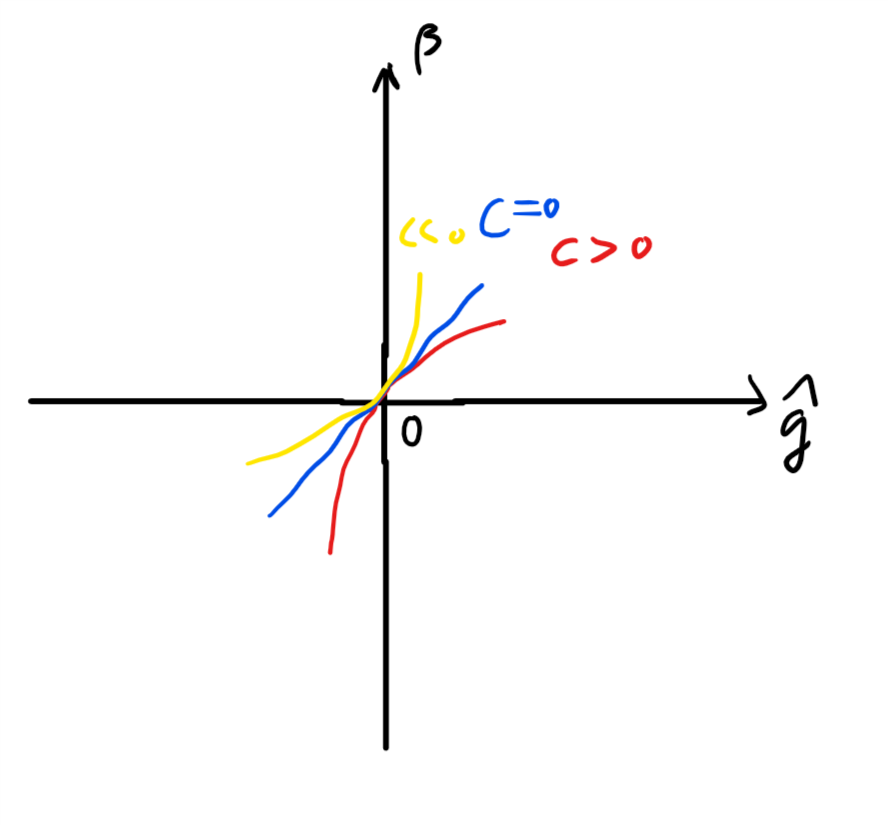
\includegraphics[scale=0.5]{PIC/hw8pic1.png}
\end{figure}
To solve equation
\begin{equation}
	\frac{d\hat{g}}{d\lambda} = - \pi C \hat{g}^2
\end{equation}
we separate variables
\[
- \frac{1}{\hat{g}^2} d \hat{g} = \pi C \lambda d\lambda
\]
Taking integrals of both sides, we get
\begin{equation}
\frac{1}{\hat{g}} = \pi C\lambda +K
\end{equation}
where $K$ is constant. When $\lambda=0$, $\hat{g} = g_*$, so $K = \frac{1}{g^*}$. Therefore,
\[
\hat{g}(\lambda) = \frac{g^*}{g^* \pi C \lambda +1}
\]
Since the $\beta$-function is
\[ 
\beta(\hat{g}) = - \pi C \hat{g}^2
\]
if $C < 0$, then $\beta > 0$, so $\mathcal{O}$ is marginal relevant. If $C=0$, then $\mathcal{O}$ is exactly marginal. If $C > 0$, then $\mathcal{O}$ is marginal irrelevant

\newpage
\section{Homework 9}
\subsection{$SU(2)$ current algebra with level 1}
\subsubsection{}
For free boson, we have OPE
\[
\varphi(z)\varphi(w) \sim - \ln (z-w)
\]
Therefore, 
\begin{equation}
\begin{split}
J(z)J^{\pm}(w) &= \frac{i\partial\varphi(z)}{\sqrt{2}}:e^{\pm i \sqrt{2}\varphi(w)}:\\
&= \frac{i \partial \varphi(z)}{\sqrt{2}}: \sum_{k=0}^{\infty} \frac{(\pm i\sqrt{2})^k}{k!} \varphi^k(w):\\
& \sim \sum_{i=0}^{\infty} \frac{(\pm i\sqrt{2})^k}{k!} \frac{i}{\sqrt{2}}k \wick{\c{\partial \varphi(z)} \c{\varphi(w)} }:\varphi^{k-1}(w):\\
& \sim \frac{1}{z-w}\sum_{i=1}^{\infty} \frac{(\pm i \sqrt{2})^{k-1}}{(k-1)!} : \varphi^{k-1}(w):\\
& \sim \frac{J^{\pm}(w)}{z-w}\\
\end{split}
\end{equation}
\begin{equation}
\begin{split}
J^{+}(z)J^{-}(w)& = : e^{+i \sqrt{2}\varphi(z)}:: e^{-i \sqrt{2}\varphi(w)}:\\
& = \sum_{m=0}^{\infty} \sum_{n=0}^{\infty}\frac{(i\sqrt{2})^m}{m!} \frac{(-i \sqrt{2})^n}{n!} : \varphi^m(z):: \varphi^n(w): \\
& \sim \sum_{m=0}^{\infty}\sum_{n=0}^{\infty} \frac{(i \sqrt{2})^m}{m!} \frac{(-i \sqrt{2})^n}{n!} k! \binom{m}{k}\binom{n}{k} \left(\wick{\c{\varphi(z)} \c{\varphi(w)} } \right)^k: \varphi^{m-k}(z) \varphi^{n-k}(w):\\
& \sim \sum_{m=1}^{\infty} \sum_{n=1}^{\infty} \frac{(i \sqrt{2})^{m-k}}{ (m-k)!} \frac{(-i \sqrt{2})^{n-k}}{(n-k)!} \frac{1}{k!} \left(-2\ln(z-w) \right)^k : \varphi^{m-k}(z) \varphi^{n-k}(w):\\
		& \sim e^{-2 \ln(z-w)}:e^{i \sqrt{2}\varphi(z)} e^{-i \sqrt{2}\varphi(w)}: \\
	& \sim \frac{:J^+(z)J^- (w):}{(z-w)^2} \\
	& \sim \frac{J^+(w) J^-(w)+ \partial_w J^+(w)J^-(w)(z-w)}{(z-w)^2} \\
	& \sim \frac{1}{(z-w)^2} + \frac{i \sqrt{2}\partial_w \varphi(w) J^+(w)J^-(w)}{z-w}\\
	& \sim \frac{1}{(z-w)^2} + \frac{2J(w)}{z-w}
\end{split}
\end{equation}
and
\begin{equation}
	\begin{split}
	J(z)J(w) &= \frac{i \partial \varphi(z)}{\sqrt{2}}\frac{i \partial \varphi(w)}{\sqrt{2}}\\
	& \sim -\frac{1}{2} \wick{\c{\partial \varphi(z) } \c{\partial \varphi(w)} }\\
	& \sim \frac{1/2}{(z-w)^2}
	\end{split}
\end{equation}
\subsubsection{}
Similarly, we have 
\begin{equation}
	\begin{split}
	J^+ (z) V_\downarrow (0) & = : e^{\sqrt{2} i \varphi(z)}:: e^{- \frac{i \varphi(0)}{\sqrt{2}}}\\
	& \sim \exp{ \wick{\c{\varphi(z)} \c{\varphi(0)}}} : e^{\sqrt{2}i \varphi(z)} e^{-\frac{i \varphi(0)}{\sqrt{2}}}:\\
	&  \sim \frac{1}{z-w} e^{\frac{i \varphi(0)}{\sqrt{2}}} = \frac{V_{\uparrow}(0)}{z-w}
	\end{split}
\end{equation}
and 
\begin{equation}
\begin{split}
J^- (z) V_\uparrow (0) & = : e^{-\sqrt{2} i \varphi(z)}:: e^{\frac{i \varphi(0)}{\sqrt{2}}}\\
& \sim \exp{ \wick{\c{\varphi(z)} \c{\varphi(0)}}} : e^{-\sqrt{2}i \varphi(z)} e^{\frac{i \varphi(0)}{\sqrt{2}}}:\\
&  \sim \frac{1}{z-w} e^{\frac{-i \varphi(0)}{\sqrt{2}}} = \frac{V_{\downarrow}(0)}{z-w}
\end{split}
\end{equation}
and 
\begin{equation}
\begin{split}
J(z) V_{\uparrow,\downarrow}(0)& = \frac{i \partial \varphi(z)}{\sqrt{2}} :e^{\pm \frac{i \varphi(0)}{\sqrt{2}}}\\
&\sim \sum_{i=0}^{\infty} \frac{(\pm i\sqrt{2}/2)^k}{k!} \frac{i}{\sqrt{2}}k \wick{\c{\partial \varphi(z)} \c{\varphi(0)} }:\varphi^{k-1}(0):\\
& \sim \frac{1}{2}\frac{1}{z-w} \sum_{i=1}^{\infty} \frac{(\pm i \sqrt{2}/2)^{k-1}}{(k-1)!} : \varphi^{k-1}(0):\\
&\sim \frac{1}{2}\frac{1}{z-w} V_{\uparrow,\downarrow}(0)
\end{split}
\end{equation}
\subsubsection{}
When $R= \sqrt{2}$, the partition function becomes
\begin{equation}
\label{eq29}
	Z_{\sqrt{2}}(\tau, \bar{\tau}) = \frac{1}{|\eta(\tau)|^2} \sum_{m,n} q^{\frac{1}{2} \frac{(m+n)^2}{2}} \bar{q}^{\frac{1}{2}\frac{(m-n)^2}{2}}
\end{equation}
$m+n$ and $m-n$ have same parity, so if they are odd, let $m+n = 2k_1 +1, m-n = 2k_2 +1$, then we have 
\begin{equation}
q^{\frac{1}{2} \frac{(m+n)^2}{2}} \bar{q}^{\frac{1}{2} \frac{(m-n)^2}{2}} = q^{(k_1 + \frac{1}{2})^2}\bar{q}^{(k_2 + \frac{1}{2})^2}
\end{equation}
if they are even, let $m+n = 2k_1, m-n = 2k_2 $, then we have 
\begin{equation}
	q^{\frac{1}{2} \frac{(m+n)^2}{2}} \bar{q}^{\frac{1}{2} \frac{(m-n)^2}{2}} = q^{k_1^2} \bar{q}^{k_2^2}
\end{equation}
Now, equation \ref{eq29} becomes
\begin{equation}
	\frac{1}{|\eta(\tau)|^2} \sum_{k_1,k_2}\left(q^{(k_1 + \frac{1}{2})^2} \bar{q}^{(k_2 + \frac{1}{2})^2} + q^{k_1^2}\bar{q}^{k_2^2}  \right)
\end{equation}
It is 
\begin{equation}
	Z_{\sqrt{2}}(\tau, \bar{\tau}) = |\chi_{\frac{1}{2}}(q)|^2 + |\chi_0 (q)|^2
\end{equation}
\subsection{$SU(2)$ current algebra with level $k$}
We have OPE of energy-momentum tensor $T$ and $J^a$ as follows
\begin{equation}
\label{eq34}
	\begin{split}
	T(z) J^a(w) & = \frac{1}{k+2} \sum_{m=1}^3 : J^m J^m (z):J^a(w)\\
	& \sim \frac{1}{k+2} \sum_{m=1}^3 : J^m(z) \wick{\c{J^m(z)} : \c{J^a(w)} }\\
	& \sim \frac{1}{k+2} \sum_{m=1}^3 : J^m(z): \left(\delta_{ma}\frac{k/2 }{(z-w)^2} + \frac{i \epsilon^{ma}_c J^c(w)}{z-w} \right)\\
	& \sim \frac{1}{k+2} \left(\frac{J^a(z)k/2}{(z-w)^2} + \frac{i \epsilon^{a}_{mc} J^c(w) }{z-w} \right)\\
	& \sim \frac{k}{2(k+2)} \left(\frac{J^a(w) + \partial_wJ^a(w)(z-w) }{(z-w)^2} \right) + \frac{1}{k+2}\left( \frac{i \epsilon^{a}_{mc}J^m(w)J^c(w) }{z-w} \right)
	\end{split}
\end{equation}
Therefore, it conformal dimension is $\frac{k}{2(k+2)}$. Let $h= \frac{k}{2(k+2)}$. We have 
\[
[L_n, J^a_m] = \frac{1}{(2\pi i)^2} \int_0 \D w w^{m+1} \int_w \D z z^{n+1} T(z) J^a(w)
\]
Taking the expression \ref{eq34} of $T(z)J^a(w)$ in it, we obtain
\begin{equation}
	\begin{split}
	[L_n,J^a_m]&= \frac{1}{(2\pi i)^2} \int_0 \D w w^{m+1} \int_{w} \D z z^{n+1} \left\{\frac{h J^a(w)}{(z-w)^2} + \frac{h\partial_w J^a(w) + 1/(k+2) i \epsilon^a_{mc}J^m(w)J^c(w)}{z-w} + \text{regular part}\right\}
	\end{split}
\end{equation}
However, we have 
\begin{equation}
	z^{n+1} = w^{n+1} + \binom{n+1}{1}(z-w) w^n + \binom{n+1}{2}(z-w)^2 w^{n-1} + \cdots + (z-w)^{n+1}
\end{equation}
Therefore, 
\begin{equation}
	\begin{split}
	&\frac{1}{2\pi i}\int_{w} \D z z^{n+1} \left\{\frac{h J^a(w)}{(z-w)^2} + \frac{h\partial_w J^a(w) + 1/(k+2) i \epsilon^a_{mc}J^m(w)J^c(w)}{z-w} + \text{regular part}\right\}\\
	&= h(n+1) w^n J^a(w) + w^{n+1} \left(  h\partial_w J^a(w) + 1/(k+2) i \epsilon^a_{mc}J^m(w)J^c(w) \right)
	\end{split}
\end{equation}
Hence
\begin{equation}
	\begin{split}
	[L_n,J^a_m]&= \frac{1}{2\pi i}\int_0 \D w \left\{h(n+1) w^{n+m+1} J^a(w) + w^{n+m+2} \left(  h\partial_w J^a(w) + 1/(k+2) i \epsilon^a_{bc}J^b(w)J^c(w) \right) \right\}\\
	&= h(n+1) J^a_{n+m} -h(n+m+2) J^a_{n+m} + \frac{i}{k+2}\epsilon^a_{bc}(J^b J^c)_{n+m+1}\\
	& = h(-m-1)J^a_{n+m} + \frac{i}{k+2}\epsilon^a_{bc}(J^b J^c)_{n+m+1}
	\end{split}
\end{equation}
Now we compute the TT OPE 
\begin{equation}
\begin{split}
T(z)T(w)&= \frac{1}{(k+2)^2} \sum_{a=1,b=1}^3 :J^aJ^a(z)::J^bJ^b(w):\\
&\sim \frac{1}{(k+2)^2} \sum_{a=1,b=1}^3 \left\{4: \wick{J^a(z)\c{J^a(z)}\c{J^b(w)} J^b(w): + \c1{J^a(z)} \c2{J^a(z)} \c2{J^b(w)} \c1{J^b(w)}  } \right\} \\
&\sim \frac{1}{(k+2)^2} \sum_{a=1,b=1}^3 \frac{k^2/4 \delta^{ab}}{(z-w)^4} + \frac{ik \delta^{ab}\epsilon^{ab}_c J^c(w)}{(z-w)^3} + \frac{2k \delta^{ab}J^a(z) + \cdots}{(z-w)^2}
\end{split}
\end{equation}
Hence its central charge is $\frac{3k^2}{2(k+2)^2}$.
\subsection{Wakimoto construction}
For bosonic field $a(z)$ we have
\begin{equation}
	a(z)a(w) \sim \frac{\kappa/2}{(z-w)^2}
\end{equation}
\begin{eqnarray}
&a'(z)a(w) \sim  \frac{- \kappa}{(z-w)^3}\\
&a(z)a'(w) \sim \frac{\kappa}{(z-w)^3}
\end{eqnarray}
and 
\begin{equation}
	a'(z)a'(w) \sim \frac{-3\kappa}{(z-w)^4}
\end{equation}
For boson field $\beta$ and $\gamma$, we have
\begin{eqnarray}
	& \beta(z) \gamma(w) \sim \frac{1}{z-w} \\
	& \beta'(z) \gamma(w) \sim \frac{-1}{(z-w)^2}\\
	& \beta(z) \gamma'(w) \sim \frac{1}{(z-w)^2} \\
	& \beta'(z) \gamma'(w) \sim \frac{-2}{(z-w)^3} 
\end{eqnarray}
\subsubsection{}
We have following OPEs
\begin{equation}
	\begin{split}
	E(z)H(w) & = - \beta(z) \left(:\gamma(w)\beta(w): + a(w) \right)\\
	& \sim - \wick{\c{\beta(z)}: \c{\gamma(w)} \beta(w): + \c{\beta(z)} \c{a(w)} } \\
	& \sim - \frac{E(w)}{z-w}
	\end{split}
\end{equation}
\begin{equation}
	\begin{split}
	E(z)F(w) & = - \beta(z) : \gamma(w)^2 \beta(w): + 2 \beta(z)\gamma(w)a(w) + k \beta(z) \gamma'(w)\\
	& \sim -2 \wick{\c{\beta(z)} :\c{\gamma(w)} \gamma(w) \beta(w): + 2 \c{\beta(z)} \c{\gamma(w)} a(w) + k \c{\beta(z)} \c{\gamma'(w)} }\\
	& \sim \frac{-2 :\gamma(w)\beta(w):}{z-w} + \frac{2a(w)}{z-w} + \frac{k}{(z-w)^2}\\
	& \sim \frac{2\left(a(w)- :\gamma(w)\beta(w): \right)}{z-w} + \frac{k}{(z-w)^2} \\
	& \sim \frac{2H(w)}{z-w} + \frac{k}{(z-w)^2}
	\end{split}
\end{equation}
\begin{equation}
	\begin{split}
	H(z)H(w)& = \left\{-: \gamma(z)\beta(z): + a(z) \right\} \left\{- : \gamma(w)\beta(w): + a(w) \right\}\\
	& = : \gamma(z)\beta(z):: \gamma(w)\beta(w): + a(z)a(w)\\
	& \sim \wick{: \c{\gamma(z)} \beta(z) \gamma(w) \c{\beta(w)}: + : \gamma(z) \c{\beta(z)} \c{\gamma(w)} \beta(w): + : \c1{\gamma(z)} \c2{\beta(z)} \c2{\gamma(w)} \c1{\beta(w)}: + \frac{\kappa/2}{(z-w)^2} }\\
	& \sim \frac{2\beta(w)\gamma(w)}{z-w} + \frac{-1+ \kappa/2}{(z-w)^2}\\
	\end{split}
\end{equation}
\begin{equation}
	\begin{split}
	H(z)F(w) & = \left\{-:\gamma(z)\beta(z): + a(z) \right\} \left\{-: \gamma(w)^2 \beta(w): + 2\gamma(w)a(w) +k \gamma'(w) \right\}\\
	& = : \gamma(z)\beta(z)::\gamma(w)^2\beta(w): -2 : \gamma(z)\beta(z):\gamma(w)a(w) - k:\gamma(z)\beta(z): \gamma'(w) + 2\gamma(w) a(z)a(w)\\
	& \sim \wick{2:\gamma(z) \c{\beta(z)}\c{\gamma(w)} \gamma(w)\beta(w): + : \c{\gamma(z)} \beta(z)\gamma(w)^2 \c{\beta(w)}: + 2 : \c1{\gamma(z)} \c2{\beta(z)}\c2{\gamma(w)} \gamma(w) \c1{\beta(w)}:}\\
	&  \wick{- 2: \gamma(z)\c1{\beta(z)} \c1{\gamma(w)}: a(w) - k : \gamma(z)\c1{\beta{z}} \c1{\gamma'(w)} + \frac{\kappa\gamma(w)}{(z-w)^2} }\\
	& \sim \frac{2: \gamma(z)\gamma(w)\beta(w):}{z-w} - \frac{\beta(z) \gamma(w)^2}{z-w} - \frac{2\gamma(w)}{(z-w)^2} - \frac{2: \gamma(z): a(w)}{z-w} - \frac{k: \gamma(z):}{(z-w)^2} + \frac{\kappa \gamma(w)}{(z-w)^2} \\
	\end{split}
\end{equation}
Since $\kappa = k+2$, we have 
\begin{equation}
	\begin{split}
	H(z)F(w) & = \frac{\gamma(w)^2\beta(w) - 2 \gamma(w)a(w)}{z-w} - \frac{k\gamma'(w)}{z-w}\\
	& = \frac{- F(w)}{z-w}\\
	\end{split}
\end{equation}
and 
\begin{equation}
	\begin{split}
	F(z)F(w) &= \left\{- : \gamma(z)^2\beta(w): + 2 \gamma(z)a(z) + k\gamma'(z) \right\} \left\{-:\gamma(w)^2\beta(w): + 2\gamma(w)a(w) + k\gamma'(w) \right\}\\
	& \sim 2: \gamma(z)^2 \wick{\c{\beta(z)} \c{\gamma(w)} \gamma(w)\beta(w): + 2 : \gamma(z)\c{\gamma(z)} \beta(z)\gamma^2(w) \c{\beta(w)}: -2: \gamma(z)^2 \c1{\beta(z)}: \c1{\gamma(w)} a(w) - k : \gamma(z)^2 \c1{\beta(z)} : \c1{\gamma'(w)}}\\
	&\wick{ - 2 \c1{\gamma(z)} a(z): \gamma(w)^2 \c1{\beta{w}}: -2 k \c1{\gamma'(z)}: \gamma(w)^2 \c1{\beta{w}}: + 4 \gamma(z)a(z)a(w)\gamma(w) + : \gamma(z)\c1{\gamma(z)} \c2{\beta(z)} \c2{\gamma(w)} \gamma(w) \c1{\beta(w)}: }\\
	& \sim \frac{2:\gamma(z)^2 \gamma(w) \beta(w):- 2: \gamma(z)\beta(z) \gamma^2(w): - 2: \gamma(z)^2: a(w)}{z-w}\\
	& - \frac{: \gamma(z)^2:}{(z-w)^2} + \frac{2a(z): \gamma(w)^2:}{z-w} - \frac{2k: \gamma(w)^2:}{(z-w)^2} - \frac{:\gamma(z)\gamma(w):}{(z-w)^2} + \frac{2\kappa:\gamma(z)\gamma(w):}{(z-w)^2}\\
	& \sim \frac{- : \gamma(z)^2: - 2k:\gamma(w)^2: - :\gamma(z)\gamma(w): + 2\kappa\gamma(z)\gamma(w)}{(z-w)^2}\\
	& \sim \frac{(3 - 2\kappa)\gamma'(w)\gamma(w)}{z-w}
	\end{split}
\end{equation}
\subsubsection{}
We have following OPEs
\begin{equation}
	\begin{split}
	T(z)E(w) & = : \frac{1}{\kappa}\left\{a(z)^2 - a'(z)  \right\} + \beta(z)\gamma'(z): \beta(w)\\
	& \sim \wick{: \beta(z) \c{\gamma^{\prime}(z)}: \c{\beta(w)} }\\
	& \sim \frac{\beta(z)}{(z-w)^2}\\
	& \sim \frac{E(w)}{(z-w)^2} + \frac{\partial_w E(w)}{z-w}\\
	\end{split}
\end{equation}
\begin{equation}
\begin{split}
T(z)H(w) &= : \frac{1}{\kappa} \left\{ a(z)^2 - a'(z) \right\} + \beta(z) \gamma'(z) : \left\{- : \gamma(w)\beta(w): + a(w) \right\}\\
& \sim \frac{1}{\kappa}\wick{2: a(z)\c{a(z)}: \c{a(w)}- \frac{1}{\kappa}: \c{a'(z)}: \c{a(w)}- : \c{\beta(z)}\gamma'(z) \c{\gamma(w)} \beta(w): }\\
& \wick{- : \beta(z) \c{\gamma'(z)} \gamma(w) \c{\beta{w}}: - : \c1{\beta(z)} \c2{\gamma'(z)} \c1{\gamma(w)} \c2{\beta(w)} }\\
& \sim \frac{(a(z))}{(z-w)^2} + \frac{1}{(z-w)^3} - \frac{:\gamma'(z) \beta(w):}{z-w} - \frac{:\beta(z) \gamma(w):}{(z-w)^2} - \frac{1}{(z-w)^3} \\
& \sim \frac{a(w) - \beta(w)\gamma(w)}{(z-w)^2} - \frac{:\gamma'(z)\beta(w):}{(z-w)} - \frac{:\beta(z)\gamma(w):}{(z-w)^2} - \frac{1}{(z-w)^3} \\
& \sim \frac{H(w)}{(z-w)^2} + \frac{\partial_wH(w)}{z-w}\\
\end{split}
\end{equation}
and 
\begin{equation}
	\begin{split}
	T(z)F(w) &= : \frac{1}{\kappa} \left\{ a(z)^2 - a'(z) \right\} + \beta(z)\gamma'(z): \left(-2 : \gamma(w)^2 \beta(w): + 2 \gamma(w)a(w) + k \gamma'(w) \right)\\
	& = : \frac{2}{\kappa} \left\{a(z)^2 - a'(z) \right\}: \gamma(w) a(w) - 2 : \beta(z)\gamma'(z): : \gamma(w)^2\beta(w): + 2 : \beta(z) \gamma'(z): \gamma(w) a(w) + k :\beta(z) \gamma'(z): \gamma'(w)\\
	& \sim \wick{ \frac{4}{\kappa} : a(z) \c{a(z)}:\gamma(w) \c{a(w)} - \frac{2}{\kappa} \c{a'(z)}: \gamma(w) \c{a(w)}: - 4 :\c{\beta(z)} \gamma'(z) \gamma(w) \c{\gamma(w)} \gamma(w) \beta{w}:  }\\
	& \wick{-2: \beta(z) \c{\gamma'(z)} \gamma(w)^2 \c{\beta(w)}: - 4 : \c1{\beta(z)} \c2{\gamma'(z)} \c1{\gamma(w)} \gamma(w) \c2{\beta(w)} + 2 : \c{\beta(z)} \gamma'(z): \c{\gamma(w)} a(w) + k : \c{\beta(z)} \gamma'(z): \c{\gamma'(w)} }\\
	& \sim \frac{2a(z)\gamma(w)}{(z-w)^2} + \frac{4 \gamma(w)}{(z-w)^3} - \frac{4: \gamma'(z)\gamma(w) \beta(w):}{z-w} - \frac{2: \beta(z) \gamma(w)^2:}{(z-w)^2} - \frac{4 \gamma(w)}{(z-w)^3} + \frac{2\gamma'(z)a(w)}{z-w} + \frac{k\gamma'(z)}{(z-w)^2}\\
	& \sim \frac{F(w)}{(z-w)^2} + \frac{\partial_w F(w)}{z-w}
	\end{split}
\end{equation}
Now, we can conclude that their conformal dimension are all $1$.
Next, we compute the TT OPE of this energy-momentum tensor
\begin{equation}
	\begin{split}
	T(z)T(w) & = \frac{1}{\kappa}\left\{a(z)^2 - a'(z) \right\}+ \beta(z) \gamma'(z)::\frac{1}{\kappa} \left\{a(w)^2 -a'(w) \right\} + \beta(w) \gamma'(w):\\
	& \sim 
	\frac{1}{\kappa^2}:: a(w)^2 -a'(w): + : \beta(z)\gamma'(z):: \beta(w) \gamma'(w): \\
	& \sim \frac{2}{\kappa} \frac{:a(z)a(w):}{(z-w)^2} + \frac{1}{4} \frac{1}{(z-w)^4}  - \frac{-3}{\kappa} \frac{1}{(z-w)^4} + \frac{:\beta(z)\gamma'(w)}{(z-w)^2} + \frac{:\gamma'(z)\beta(w):}{(z-w)^2} + \frac{1}{(z-w)^4}\\
	& + \frac{2}{\kappa} \frac{a(w)}{(z-w)^3} - \frac{2}{\kappa}\frac{a(z)}{(z-w)^3}\\
	& \sim \frac{5/4 - 3/\kappa}{(z-w)^4} + \frac{2}{\kappa}\frac{a(w)-a(z)}{(z-w)^3} + \frac{\frac{2}{\kappa} : a(z)a(w): + :\beta(z)\gamma'(w): + \gamma'(z)\beta(w)}{(z-w)^2}\\
	& \sim \frac{5/4 - 3/\kappa}{(z-w)^4} + \frac{2T(w)}{(z-w)^2} - \frac{\partial_w T(w)}{z-w}
	\end{split}
\end{equation}
So its central charge is $\frac{5}{2} - \frac{6}{\kappa}$.
Next, we calculate the OPE of $T$ and $V_\alpha$ to compute conformal dimension of $V_\alpha(z)$.
\begin{equation}
	\begin{split}
	T(z)V_\alpha(w)& = T(z): \exp \left(i\alpha \sqrt{2/\kappa} \varphi(w) \right): \\
	&\sim \wick{i \alpha \sqrt{\frac{2}{\kappa}}\c1{T(z)} \c1{\varphi(w)} : \exp\left(i \alpha \sqrt{2/\kappa}\varphi(w) \right): }
	\end{split}
\end{equation}
because there is relation
\[
\wick{ \c{T(z)} :\c{\exp(A(w))}: = \c{T(z)} \c{A(z)} : \exp(A(z)) }
\]
Therefore, we just need to calculate $T(z)\varphi(w)$
\begin{equation}
	\begin{split}
	T(z)\varphi(w)& = \frac{1}{\kappa}: \left\{a(z)^2 - a'(z) \right\} \varphi(w)\\
	&\sim \wick{\frac{2}{\kappa} : a(z) \c{a(z)} : \c{\varphi(w)} - \frac{1}{\kappa}: \c{a'(z)}: \c{\varphi(w)} } \\
	& \sim - i \sqrt{\frac{2}{\kappa}}\left\{ \frac{a(z)}{z-w} + \frac{1/2}{(z-w)^2}  \right\}
	\end{split}
\end{equation}
Hence
\begin{equation}
	\begin{split}
	T(z)V_\alpha(w) & \sim \frac{2\alpha/\kappa V_\alpha (w)a(w)}{z-w} + \frac{\alpha/\kappa V_\alpha(w)}{(z-w)^2}
	\end{split}
\end{equation}
Hence conformal dimension of $V_\alpha$ is $\alpha/\kappa$.
\subsubsection{}
\begin{equation}
	E(z)V_{\alpha=-1}(w) = \beta(z)\exp{-i \sqrt{2/k} \varphi(w)}\beta(w) \sim 0
\end{equation}
\begin{equation}
\begin{split}
	H(z)V_{\alpha =-1}(w) &= \left\{ -: \gamma(z)\beta(z): + a(z) \right\}: e^{-i \sqrt{2/\kappa} \varphi(w)}\beta(w):\\
	& \sim \wick{- : \c{\gamma(z)}\beta(z) \exp(-i\sqrt{2/k}) \c{\beta(w)}: + \c{a(z)} : \c{\exp(-i \sqrt{2/k} \varphi(w))} \beta(w): }\\
	& \sim \frac{\beta(z) \exp( -i \sqrt{2/\kappa}\varphi(w) )}{z-w} + \frac{- \exp(-i\sqrt{2/\kappa} \varphi(w))\beta(w)}{z-w}\\
	& \sim 0
\end{split}
\end{equation}
and
\begin{equation}
	\begin{split}
	H(z)V_{\alpha=-1} &= - : \gamma(z)^2 \beta(z): e^{-i \sqrt{2/\kappa}\varphi(w)} \beta(w) + 2\gamma(z)a(z) e^{-i \sqrt{2/\kappa}\varphi(z)} \beta(w) + k \gamma'(z) e^{i \sqrt{2/\kappa}\varphi(w)} \beta(w)\\
	& \sim -2 \wick{:\gamma(z) \c{\gamma(z)} \beta(z): \c{\beta(w)} e^{-i\sqrt{\frac{2}{\kappa}}} + 2 \c{\gamma(z)} a(z) \exp(-i \sqrt{2/\kappa} \varphi(w)) \c{\beta(z)}}\\
	& + \wick{\gamma(z) \c{a(z)} \c{\exp(-i \sqrt{2/\kappa}\varphi(w))} \beta(w) + \c1{\gamma(z)} \c2{a(z)} \c2{\exp(-i \sqrt{2/\kappa}\varphi(w))} \c1{\beta(w)} + k \c{\gamma'(z)} \c{\beta(w)}e^{-i \sqrt{2/\kappa}\varphi(w)} }\\ 
	& \sim \frac{(k+2)e^{-i \sqrt{2/\kappa} \varphi(w)}}{(z-w)^2} - \frac{2 a(w) e^{-i \sqrt{2/\kappa}\varphi(w)}}{z-w}
	\end{split}
\end{equation}
and 
\begin{equation}
	\begin{split}
	T(z)V_{\alpha=-1} & = T(z)V_{-1}(w)\beta(w)\\
	& \sim \wick{ \c{T(z)} \c{V_{-1}(w)} \beta(w) + \c{T(z)}V_{-1}(w) \c{\beta(w)} }\\
	& \sim \frac{\partial_w (V_{\alpha =-1})}{z-w} + \frac{(1-1/\kappa)V_{\alpha=-1}(w)}{(z-w)^2}
	\end{split}
\end{equation}
Next, we only need to prove $[L_n, V_{\alpha=-1}]=0$.

However
\begin{equation}
	\begin{split}
	[L_n,V_{\alpha=-1}] &= \frac{1}{2\pi i}\int_0 \D w \int_w \D z z^{n+1} T(z) V_{\alpha=-1}(w)\\
	&= \int_0 \D w \partial_w \left(w^{n+1}V_{\alpha=-1}(w) \right) - \frac{n+1}{\kappa}V_{\alpha=-1}(w)\\
	&=0
	\end{split}
\end{equation}
Hence $V_{\alpha=-1}$ is screening current.
% !TEX root=../main.tex
% !TEX program=luatex
\newpage
\section{Homework 10}
\subsection{Derivation}
\[
 \Gamma = \frac{-i}{12 \pi} \int_B \D^3 y \epsilon_{\alpha\beta\gamma} \tr( \tilde{g}^{-1} \partial^a \tilde{g} \tilde{g}^{-1} \partial^{\beta} \tilde{g} \tilde{g}^{-1} \partial^\gamma \tilde{g})
\]
we have with integration by parts
\begin{equation}
	\begin{split}
	\Gamma & = \frac{-i}{12 \pi} \int_B \D^3 y \epsilon_{\alpha\beta\gamma} \tr\left( \tilde{g}^{-1} \partial^\gamma \left( \partial^\alpha \tilde{g} \tilde{g}^{-1} \partial^\beta \tilde{g}\right) \right) + \frac{i}{4\pi} \int_\Sigma \D^3 x \epsilon_{\mu \eta} \tr \left( \partial^{\mu} \tilde{g} \tilde{g}^{-1} \partial^{\eta} \tilde{g} \tilde{g}^{-1} \right)\\
	& =  \frac{-i}{12 \pi} \int_B \D^3 y \epsilon_{\alpha\beta\gamma} \tr\left( \tilde{g}^{-1} \partial^\gamma \left( \partial^\alpha \tilde{g} \tilde{g}^{-1} \partial^\beta \tilde{g}\right) \right) - \frac{i}{4 \pi} \int_{\Sigma} \D^2 x \epsilon_{\mu\eta} \tr\left( \partial^{\mu} g \partial^{\eta} g^{-1}\right)
	\end{split}
\end{equation}
The second term is independent of $g$, therefore the derivative by $g$ is
\begin{equation}
	\begin{split}
	\delta \Gamma & = \frac{i}{4\pi} \int_{\Sigma}\D^2 x \epsilon_{\mu\eta} \tr \left(\delta g^{-1} \partial^{\mu} g g^{-1} \partial^{\mu} g \right)\\
	& = \frac{-i}{4\pi} \int_{\Sigma} \D^2 x \epsilon_{\mu\eta} \tr \left( \delta g^{-1} g \partial^{\mu} (g^{-1} \partial^{\mu} g) \right)\\
	& = \frac{i}{4\pi} \int_{\Sigma} \D^2 x \epsilon_{\mu\eta} \tr \left(  g^{-1} \delta g \partial^{\mu} (g^{-1} \partial^{\mu} g) \right)
	\end{split}
\end{equation}
with $\delta(g g^{-1})=0$.
\subsection{Solutions to KZ equations}
\subsubsection{}
All possible generators of $\square^{\otimes2}$ is 
\[
\begin{aligned}
|+,+\rangle & & |+,- \rangle & & |-,+\rangle & & |-,-\rangle
\end{aligned}
\]
since we have anti-symmetry relation $|+,-\rangle = -|-,+\rangle$, $|+,-\rangle$ is the generator of trivial one-dimensional representation $\mathbf{1}$. And ${\tiny\yng(2)}$ is 2-dimensional representation with generators $|+,+\rangle$ and $|-,-\rangle$.

Let us consider the generator of ${\tiny\yng(2)} \otimes {\tiny\yng(1)}$. It has generator
\[
\begin{aligned}
&|+,+,+\rangle& & |-,-,+\rangle& & |+,-,+\rangle\\
&|+,+,-\rangle& & |-,-,-\rangle& & |+,-,-\rangle
\end{aligned}
\]
since $|-,-,+\rangle \sim |+,-,-\rangle \sim |-\rangle$ and $|+,-,+ \rangle \sim |+,+,-\rangle \sim |+\rangle$,, where $\sim$ means linear equivalence, we can conclude that 
\begin{equation}
	{\tiny\yng(2)} \otimes {\tiny\yng(1)} \cong {\tiny\yng(3)} \oplus {\tiny\yng(1)}
\end{equation}
Hence
\begin{equation}
	(\square)^{\otimes 3} \cong \left( {\tiny\yng(2)} \oplus \mathbf{1} \right) \otimes {\tiny\yng(1)} \cong {\tiny\yng(3)} \oplus {\tiny\yng(1)} \oplus {\tiny\yng(1)}
\end{equation}
\begin{equation}
	\begin{split}
	(\square)^{\otimes 4} &\cong \left({\tiny\yng(3)} \otimes {\tiny\yng(1)}\right) \oplus {\tiny\yng(2)}^{\oplus 2} \oplus \mathbf{1}^{\oplus 2}\\
	&\cong {\tiny\yng(4)} \oplus {\tiny\yng(2)}^{\oplus 3} \oplus \mathbf{1}^{\oplus 2}
	\end{split}
\end{equation}
and
\begin{equation}
	\begin{split}
	(\square)^{\otimes 5} &\cong \left({\tiny\yng(4)} \otimes {\tiny\yng(1)}\right) \oplus \left({\tiny\yng(2)} \otimes {\tiny\yng(1)}\right)^{\oplus 3} \oplus {\tiny\yng(1)}^{\oplus 2}\\
	&\cong {\tiny\yng(5)} \oplus {\tiny\yng(3)}^{\oplus 4} \oplus {\tiny\yng(1)}^{\oplus 5}
	\end{split}
\end{equation}
\subsubsection{}
\subsubsection{}
The KZ equations 
\begin{equation}
	\left[ \partial_{z_1} + \frac{2}{k+2} \sum^n_{j=2} \frac{\Omega_{1j}}{z_1 - z_j} \right] \Phi_{\frac{n-2}{2}} (z_1, \cdots, z_n) =0
\end{equation}
We have 
\begin{equation}
	\begin{split}
	\partial_{z_1} \Phi_{\frac{n-2}{2}} & = \partial_{z_1} \psi_0 \sum_{i\geq 1}^{n} \psi_i |v_i \rangle\\
		& = \left( \partial_{z_1} \psi_0 \right) \sum_{i \geq 1}^n \psi_i |v_i \rangle + \psi_0 \partial_{z_1}\left( \sum_{i \geq 1}^{n} \psi_i |v_i \rangle \right)\\
	\end{split}
\end{equation}
Since we have 
\begin{equation}
\partial_{z_1 } \psi_0 = - \frac{2}{k+2} \sum_{j \geq 2} \frac{1/4}{z_1 -z_j} \sum_{i \geq 1}^n \psi_i
\end{equation}
we have 
\begin{equation}
\begin{split}
 \partial_{z_1} \Phi_{\frac{n-2}{2}} = \psi_0 \left\{ - \frac{2}{k+2} \sum_{j \geq 2}^n \frac{1/4}{z_1 - z_j}  + \partial_{z_1} \right\}\sum_{i \geq 1}^n \psi_i |v_i \rangle
\end{split}
\end{equation}
if $\psi_0 \neq 0$, they reduce
\begin{equation}
\label{eq67}
	\left[ \partial_{z_1} + \frac{2}{k+2} \sum^n_{j=2} \frac{\Omega_{1j}-1/4 }{z_1 - z_j} \right] \sum_{i=1}^{n}\psi_i(z)|v_i \rangle
\end{equation}

In general, the result in previous part implies
\[
\Omega_{ij} = \frac{1}{2}(s_{ij} -\frac{1}{2}) \text{ if }  i \neq j
\]
In particular, we have 
\begin{eqnarray}
& \Omega_{1j} \left| v_1 \right\rangle = \frac{1}{2}| v_j\rangle - \frac{1}{4}\left| v_1 \right\rangle \\
& \Omega_{1j} \left| v_j \right\rangle = \frac{1}{2}|v_1 \rangle - \frac{1}{4}|v_j\rangle 
\end{eqnarray}
Therefore, the coefficient of $|v_1 \rangle$  of $\ref{eq67}$ is 
\begin{equation}
	\partial_{z_1 } \psi_1 + \frac{2}{k+2} \sum_{j=2}^n \frac{-1/2 \psi_1}{z_1 -z_j} + \frac{2}{k+2} \sum_{j=2}^n \frac{1/2 \psi_j}{z_1 - z_j}
\end{equation}
where the middle term comes form $\Omega_{1j} |v_1\rangle$ and the last term comes from $\Omega_{1j} |v_j \rangle$. The KZ equations implies this coefficient is equal to zero. Hence
\begin{equation}
	(k+2) \partial_{z_1} \psi_1 + \sum_{j=2}^n \frac{\psi_j - \psi_1}{z_1 - z_j} =0 
\end{equation}
Similarly, the coefficient of \ref{eq67} is 
\begin{equation}
	\partial_{z_1} \psi_2 + \frac{2}{k+2} \frac{1/2 \psi_1}{z_1 - z_2} + \frac{2}{k+2} \frac{-1/2 \psi_2}{z_1 - z_2}
\end{equation}
The middle term comes from $\Omega_{12} | v_1 \rangle$ and the last term comes from $\Omega_{12} | v_2 \rangle$. Therefore, we get
\begin{equation}
(k+2) \partial_{z_1} \psi_2 + \frac{\psi_1 - \psi_2}{z_1 - z_2} =0
\end{equation}
\newpage
\section{Homework 11}
\subsection{Modular transformation of the $\theta$ and $\eta$ functions}
\subsubsection{}
Since the period of $\varphi$ is $2\pi R$, that is $\varphi = \varphi +  2 \pi R n$ for all $n \in \mathbb{Z}$, therefore in particular
\begin{equation}
	:e^{i\alpha \varphi}: = : e^{i \alpha (\varphi+ 2 \pi R)}: = : e^{i \alpha \varphi}: e^{2 \pi i \alpha R}
\end{equation}
It implies that $\alpha R \in \mathbb{Z}$ since $e^{2\pi i \alpha R}=1$. Conversely, if $\alpha R = m$ for some integer $m$, then for any integer $n$, we have 
\begin{equation}
	:e^{i\alpha(\varphi + 2n \pi R)}: = :e^{i \alpha \varphi}: e^{i m 2n \pi}: = :e^{i\alpha \varphi}
\end{equation}
Hence all possible value of $\alpha$ is $\frac{m}{R}\ m \in \mathbb{Z}$.
\subsubsection{}
We have commutation relations $[L_0, \bar{\psi}_r] = - r \bar{\psi}_r$ and $[L_0, \psi_r] = -r \psi_r$. Hence
\begin{equation}
	\begin{split}
	 L_0 \left(\psi_{-\frac{k}{2}} \right)^{n_{k/2}} & = \left([L_0, \psi_{-\frac{k}{2}}] + \psi_{-\frac{k}{2}} L_0 \right) \left( \psi_{-\frac{k}{2}} \right)^{n_{k/2}-1}\\
	 & =\frac{k}{2}\left( \psi_{-\frac{k}{2}} \right)^{n_{k/2}} + \psi_{-\frac{k}{2}}L_0 \left(\psi_{-\frac{k}{2}} \right)^{n_{k/2}-1}\\
	 & =\frac{k}{2} n_{k/2} \left(\psi_{-\frac{k}{2}} \right)^{n_{k/2}} + \left( \psi_{-\frac{k}{2}} \right) ^{n_{k/2}}L_0
	\end{split}
\end{equation}
and similarly
\begin{equation}
	 L_0 \left(\bar{\psi}_{-\frac{k}{2}} \right)^{n_{k/2}} =n_{k/2} \left(\bar{\psi}_{-\frac{k}{2}} \right)^{n_{k/2}} + \left( \bar{\psi}_{-\frac{k}{2}} \right) ^{n_{k/2}}L_0
\end{equation}
Therefore, we have
\begin{equation}
	\begin{split}
	L_0 |n_1,n_2,\cdots \rangle & = \sum_{k \geq 1} \left(\frac{2k-1}{2} n_{(2k-1)/2} \right)|n_1,n_2,\cdots \rangle
	\end{split}
\end{equation}
and
\begin{equation}
	L_0 \overline{|n_1,n_2, \cdots\rangle}= \sum_{k \geq 1} \left(\frac{2k-1}{2} n_{(2k-1)/2} \right)\overline{|n_1,n_2,\cdots \rangle}
\end{equation}
For $J_0$, we have similar equations
\begin{equation}
\begin{split}
J_0 \left(\psi_{-\frac{k}{2}} \right)^{n_{k/2}} & = \left([J_0, \psi_{-\frac{k}{2}}] + \psi_{-\frac{k}{2}} J_0 \right) \left( \psi_{-\frac{k}{2}} \right)^{n_{k/2}-1}\\
& =\left( \psi_{-\frac{k}{2}} \right)^{n_{k/2}} + \psi_{-\frac{k}{2}}J_0 \left(\psi_{-\frac{k}{2}} \right)^{n_{k/2}-1}\\
& = n_{k/2} \left(\psi_{-\frac{k}{2}} \right)^{n_{k/2}} + \left( \psi_{-\frac{k}{2}} \right) ^{n_{k/2}}L_0
\end{split}
\end{equation}
\begin{equation}
\begin{split}
J_0 \left( \bar{\psi}_{-\frac{k}{2}} \right)^{n_{k/2}} =-n_{k/2} \left(\bar{\psi}_{-\frac{k}{2}} \right)^{n_{k/2}} + \left( \bar{\psi}_{-\frac{k}{2}} \right) ^{n_{k/2}}L_0	
\end{split}
\end{equation}
Therefore, we have
\begin{equation}
\begin{split}
J_0 |n_1,n_2,\cdots \rangle & = \sum_{k \geq 1} \left( n_{(2k-1)/2} \right)|n_1,n_2,\cdots \rangle
\end{split}
\end{equation}
and
\begin{equation}
J_0 \overline{|n_1,n_2, \cdots\rangle}= \sum_{k \geq 1} \left(-n_{(2k-1)/2} \right)\overline{|n_1,n_2,\cdots \rangle}
\end{equation}
We have $\{\psi_r, \psi_r\} =0$, hence all possible values of $n_{k/2}$ are $0$ and $1$. Since $L_0$ and $J_0$ are commutative, they simultaneously have eigenvalues, so
\begin{equation}
	\begin{split}
	\tr_{H_{\psi}}(q^{L_0} y^{J_0}) & = \sum_{\forall n_{j+1/2}=0,1}\langle n_1,n_2,\cdots | q^{L_0} y^{J_0} | n_1 ,n_2, \cdots \rangle \\
	& = \sum_{\forall  n_{j+1/2}=0,1} \langle n_1,n_2,\cdots | q^{\sum_{k \geq 1}(k+1/2)n_{k+1/2}} y^{n_{k+1/2}} | n_1,n_2 , \cdots \rangle\\
	& = \prod_{k \geq 1} \left( 1+ q^{k+\frac{1}{2}} y \right)
	\end{split}
\end{equation}
where $H_{\psi}$ is Hilbert space generated by $\psi$. Similarly for $H_{\bar{\psi}}$, we have trace
\begin{equation}
	\begin{split}
	\tr_{H_{\psi}}(q^{L_0} y^{J_0}) & = \sum_{\forall n_{j+1/2}=0,1}\overline{\langle n_1,n_2,\cdots |} q^{L_0} y^{J_0} \overline{| n_1 ,n_2, \cdots \rangle} \\
	& = \sum_{\forall  n_{j+1/2}=0,1} \overline{\langle n_1,n_2,\cdots |} q^{\sum_{k \geq 1}(k+1/2)n_{k+1/2}} y^{-n_{k+1/2}} \overline{| n_1,n_2 , \cdots \rangle}\\
	& = \prod_{k \geq 1} \left( 1+ q^{k+\frac{1}{2}} y^{-1} \right)
	\end{split}
\end{equation}
Combining these results and $H= H_{\psi } \otimes H_{\bar{\psi}}$ since $\psi$ and $\bar{\psi}$ are linearly independent.
\begin{equation}
	\begin{split}
	\tr (q^{L_0 - \frac{1}{24}} y^{J_0}) & = q^{-\frac{1}{24}} \tr_{H}(q^{L_0}y^{J_0})\\
	&= q^{-\frac{1}{24}} \tr_{H_\psi \otimes H_{\bar{\psi}}} \left(q^{L_0} y^{J_0} \right)\\
	& = q^{-\frac{1}{24}} \tr_{H_{\psi}}\left(q^{L_0} y^{J_0} \right) \tr_{H_{\bar{\psi}}} \left( q^{L_0} y^{J_0} \right)\\
	& = q^{-\frac{1}{24}} \prod_{n \geq 1} \left(1 + q^{n-\frac{1}{2}} y \right) \left( 1+ q^{n-\frac{1}{2}} y^{-1} \right)
	\end{split}
\end{equation}
\subsubsection{}
Now, we need to compute $L_0 J_{-1}^{n_1} J_{-2}^{n_2} \cdots $. However, we have $[L_0, J_{-n}] = n J_{-n}$, hence
\begin{equation}
	\begin{split}
	L_0 J^{n_i}_{-i} = &\left( [L_0, J_{-i}] + J_{-i}L_0 \right) (J_{-i}^{n_i})^{n_i -1} \\
	& =\left(J_{-i} + J_{-i} L_0\right)(J_{-i})^{n_i -1} \\
	& = n_i (J_{-i})^{n_i} + (J_{-i})^{n_i}L_0\\ 
	\end{split}
\end{equation}
So
\begin{equation}
	\begin{split}
	L_0 |\alpha, n_1, \cdots \rangle &= \lim_{z,\bar{z} \to 0} J_{-1}^{n_1} J_{-2}^{n_2} \cdots V_{\alpha}(z,\bar{z}) |0\rangle \\
	& = \left( \sum_{k\geq 1} k n_k + \frac{\alpha ^2}{2} \right) |\alpha, n_1, \cdots \rangle
	\end{split}
\end{equation}
and $[J_0,J_{-k}] = 0$ implies
\begin{equation}
	\begin{split}
	J_0 |\alpha, n_1, \cdots \rangle & = \lim_{z,\bar{z} \to 0} J_{-1}^{n_1} J_{-2}^{n_2} \cdots J_0 V_{\alpha} (z, \bar{z}) |0\rangle\\
	& =\alpha | \alpha, n_1 ,\cdots \rangle
	\end{split}
\end{equation}
Fix $\alpha$ we have 
\begin{equation}
	\begin{split}
	\tr_\alpha (q^{L_0 - \frac{1}{24}} y^{J_0}) &=  q^{-\frac{1}{24}}\sum_{n_1 \geq 0}\sum_{n_2 \geq 0} \cdots \prod_{k \geq 1} q^{k n_k} q^{\alpha^2/2} y^{\alpha}\\
	& = q^{-\frac{1}{24}} q^{\alpha^2/2}y^{\alpha}\prod_{k \geq 1} \sum_{n_k \geq 0} (q^k)^{n_k}\\
	& =q^{-\frac{1}{24}} q^{\alpha^2/2}y^{\alpha} \prod_{k \geq 1} \frac{1}{1- q^k}\\
	& = \frac{1}{\eta(\tau)} q^{\alpha^2/2}y^{\alpha}
	\end{split}
\end{equation}
Now 
\begin{equation}
	\begin{split}
	\tr(q^{L_0 -\frac{1}{24}} y^{J_0}) & = \sum_{\alpha} \tr_{\alpha}(q^{L_0 -\frac{1}{24}} y^{J_0})\\
	& = \sum_{\alpha = n/R} \tr_{\alpha}(q^{L_0 -\frac{1}{24}} y^{J_0})\\
	& = \frac{1}{\eta(\tau)}\sum_{n\in \mathbb{Z}} q^{n^2/2R^2}y^{n/R}
	\end{split}
\end{equation}
when $R=1$, it is our desired result.
\subsubsection{}
By definition, we have 
\begin{equation}
	\begin{split}
	\vartheta_4(\tau) & = \prod_{n\geq 1} (1-q^n) (1- q^{n-\frac{1}{2}})^2 \\
	& = q^{-\frac{1}{24}} \eta(\tau) \prod_{n \geq 1} (1- q^{n-\frac{1}{2}})^2\\
	\end{split}
\end{equation}
when $y = -1$ the Jacobi triple product identity becomes 
\begin{equation}
	\begin{split}
	q^{-\frac{1}{24}} \prod_{n \geq 1} (1- q^{n-\frac{1}{2}})^2 = \frac{1}{\eta(\tau)} \sum_{n\in \mathbb{Z}} (-1)^n q^{\frac{n^2}{2}}
	\end{split}
\end{equation}
Therefore, 
\begin{equation}
	\vartheta_4(\tau) = \sum_{n \in \mathbb{Z}} (-1)^n q^{\frac{n^2}{2}}
\end{equation}
Similarly, we have 
\begin{equation}
	\begin{split}
	\vartheta_3(\tau) & = \prod_{n \geq 1} (1-q^n)(1+ q^{n-\frac{1}{2}})^2\\
	& = \frac{1}{\eta(\tau)} \prod_{n \geq 1} (1+ q^{\frac{1}{2}})^2
	\end{split}
\end{equation}
and when $y =1$, with Jacobi triple product identity
\begin{equation}
		q^{-\frac{1}{24}} \prod_{n \geq 1} (1+ q^{n-\frac{1}{2}})^2 = \frac{1}{\eta(\tau)} \sum_{n\in \mathbb{Z}}  q^{\frac{n^2}{2}}
\end{equation}
therefore,
\begin{equation}
	\vartheta_3(\tau) = \sum_{n \in \mathbb{Z}} q^{\frac{n^2}{2}}
\end{equation}
when $y = q^{\frac{1}{2}}$, we have 
\begin{equation}
	q^{-\frac{1}{24}} \prod_{n \geq 1} (1+ q^{n})(1+ q^{n-1}) = \frac{1}{\eta(\tau)} \sum_{n\in \mathbb{Z}}  q^{\frac{n^2+n}{2}}
\end{equation}
it is equivalent to 
\begin{equation}
	2q^{-\frac{1}{24}} \prod_{n \geq 1} (1+ q^{n})^2 = \frac{1}{\eta(\tau)} \sum_{n\in \mathbb{Z}}  q^{\frac{n^2+n}{2}}
\end{equation}
therefore,
\begin{equation}
	\begin{split}
	\vartheta_2(\tau) & = 2q^{\frac{1}{8}} \prod_{n \geq 1} (1- q^n)(1+q^n)^2 \\
	& = q^{\frac{1}{8}} \sum_{n\in \mathbb{Z}} q^{\frac{n^2+n}{2}}\\
	& = \sum_{n\in \mathbb{Z}} q^{\frac{(n+1/2)^2}{2}}
	\end{split}
\end{equation}
With $T$-transformation $\tau \to \tau +1$, we have $q \to e^{2\pi i} q$, so
\begin{equation}
	\begin{split}
	\vartheta_2(\tau+1) & = \sum_{n\in \mathbb{Z}} e^{(n+1/2)^2 \pi i} q^{\frac{(n+1/2)^2}{2}}\\
	& = e^{i\pi/4} \sum_{n \in \mathbb{Z}} e^{n(n+1)\pi i} q^{\frac{(n+1/2)^2}{2}}\\
	& = e^{i\pi/4}  \vartheta_2(\tau)
	\end{split}
\end{equation}
\begin{equation}
	\begin{split}
	\vartheta_3(\tau+1) & = \sum_{n \in \mathbb{Z}} e^{n^2 \pi i}q^{\frac{n^2}{2}}\\
	& = \sum_{n \in \mathbb{Z}} (-1)^n q^{\frac{n^2}{2}} \\
	&= \vartheta_4(\tau)
	\end{split}
\end{equation}
and similarly we have $\vartheta_4(\tau +1) = \sum_{n \in \mathbb{Z}} (-1)^{2n} q^{\frac{n^2}{2}} = \vartheta_3(\tau)$. 
We have following Poisson resummation formula
\begin{equation}
	\sum_{n \in \mathbb{Z}} e^{- \pi an^2 +bn} = \frac{1}{\sqrt{a}} \sum_{k \in \mathbb{Z}} e^{- \frac{\pi}{a}\left( k + \frac{b}{2 \pi i}\right)^2 }
\end{equation}
let $a = i /\tau, b=0$, we get
\begin{equation}
\vartheta_3(- \frac{1}{\tau}) =\sum_{n \in \mathbb{Z}} e^{-\frac{2\pi i }{\tau} \frac{n^2}{2}} = \sqrt{-i \tau} \sum_{k \in \mathbb{Z}} e^{i \pi \tau k^2} = \vartheta_3(\tau)
\end{equation}
let $ a = \frac{i}{\tau}, b= \pi i$, we get 
\begin{equation}
\label{eq112}
	\vartheta_4(-\frac{1}{\tau}) = \sum_{n \in \mathbb{Z}} e^{-\frac{\pi i}{\tau} n^2 + \pi i n} = \sqrt{-i \tau} \sum_{k \in \mathbb{Z}} e^{i \pi \tau (k +1/2)^2} = \sqrt{-i \tau} \vartheta_2(\tau)
\end{equation}
Hence $\vartheta_2(-\frac{1}{\tau}) = \sqrt{\frac{\tau}{i}} \vartheta_4(\tau)$ by taking $-1/\tau$ in \ref{eq112}.
\subsubsection{}
We have
\begin{equation}
	\begin{split}
	\vartheta_2(\tau) \vartheta_3(\tau) \vartheta_4(\tau) & = 2 q^{\frac{1}{8}} \prod_{n \geq 1} (1-q^n)^3 (1-q^{2n})^2(1+q^n)^2\\
	& = 2q^{\frac{1}{8}} \prod_{n \geq 1} (1-q^n)(1-q^{2n})^2(1-q^{2n-1})^2 \\
	& =2 q^{\frac{1}{8}} \prod_{n \geq 1} (1-q^n)^2(1-q^n)\\
	& = 2q^{\frac{1}{8}} \left(\prod_{n \geq 1} (1-q^n) \right)^3
	\end{split}
\end{equation}
At the same time
\[
\eta(\tau)^3 = (q^{\frac{1}{24}} \prod_{n \geq 1} (1-q^n))^3 = q^{\frac{1}{8}} \prod_{n \geq 1} (1-q^n)^3
\]
hence we can conclude that 
\begin{equation}
	\sqrt{\frac{\vartheta_2(\tau)\vartheta_3(\tau)\vartheta_3(\tau)}{2 \eta(\tau)^3}} =1
\end{equation}
With last results, we have 
\begin{equation}
	\begin{split}
	\eta(\tau +1)^3 &= \frac{1}{2} \vartheta_2 \vartheta_3 \vartheta_4(\tau)\\
	& = \frac{1}{2} e^{i \pi} \vartheta_2 \vartheta_4 \vartheta_3 (\tau)\\
	& = e^{\frac{i \pi}{4}} \eta(\tau)^3
	\end{split}
\end{equation}
Now we can conclude that $\eta(\tau +1)= e^{\frac{i \pi}{12}} \eta(\tau)$. The $T$-transformation is similar and is equal to
\[
\eta(- \frac{1}{\tau}) = \sqrt{-i \tau} \eta(\tau)
\]
\subsection{Verlinde algebra of Ising model}
We have 
\begin{equation}
	\begin{split}
	\chi_1(- \frac{1}{\tau})& = \frac{1}{2} \left(\sqrt{\frac{\vartheta_3(-1/\tau)}{\eta(-1/\eta)}} + \sqrt{\frac{\vartheta_4(-1/\tau)}{\eta(-1/\tau)}} \right)\\
	& = \frac{1}{2} \left(\sqrt{\frac{\vartheta_3(-1/\tau)}{\eta(-1/\eta)}} + \sqrt{\frac{\vartheta_2(-1/\tau)}{\eta(-1/\tau)}} \right)\\
	& = \frac{1}{2} \left( \chi_1(\tau) + \chi_2(\tau) + \sqrt{2} \chi_3(\tau) \right)\\
	\end{split}
\end{equation}
\begin{equation}
\begin{split}
\chi_2(- \frac{1}{\tau})& = \frac{1}{2} \left(\sqrt{\frac{\vartheta_3(-1/\tau)}{\eta(-1/\eta)}} - \sqrt{\frac{\vartheta_4(-1/\tau)}{\eta(-1/\tau)}} \right)\\
& = \frac{1}{2} \left(\sqrt{\frac{\vartheta_3(-1/\tau)}{\eta(-1/\eta)}} - \sqrt{\frac{\vartheta_2(-1/\tau)}{\eta(-1/\tau)}} \right)\\
& = \frac{1}{2} \left( \chi_1(\tau) + \chi_2(\tau) - \sqrt{2} \chi_3(\tau) \right)\\
\end{split}
\end{equation}
\begin{equation}
	\begin{split}
	\chi_3(- \frac{1}{\tau}) & = \frac{1}{\sqrt{2}} \sqrt{\frac{\vartheta_2(-1/\tau)}{\eta(-1/\tau)}}\\
	& = \frac{1}{\sqrt{2}}\sqrt{\frac{\vartheta_4(-1/\tau)}{\eta(-1/\tau)}}\\
	& =\frac{\chi_1(\tau)-\chi_2(\tau)}{\sqrt{2}}
	\end{split}
\end{equation}
Therefore, the $S$-matrix is 
\begin{equation}
	S= \begin{pmatrix}
	\frac{1}{2} &\frac{1}{2} & \sqrt{2} \\
	\frac{1}{2} & \frac{1}{2} & - \sqrt{2}\\
	\frac{\sqrt{2}}{2}& -\frac{\sqrt{2}}{2}& 0\\
	\end{pmatrix}
\end{equation}
Its inverse is
\begin{equation}
	S^{-1} = \begin{pmatrix}
	\frac{2}{3} & \frac{2}{3} & \frac{\sqrt{2}}{3} \\
	\frac{1}{3} & \frac{1}{3} & - \frac{\sqrt{2}}{3} \\
	\frac{\sqrt{2}}{4} & -\frac{\sqrt{2}}{4} & 0\\
	\end{pmatrix}
\end{equation}
Taking these value in Verlinde's formula, we get
\begin{equation}
	\begin{aligned}
	N^1_{11} =1 & &N^2_{11}=0 & &N^3_{11}=0 \\
	N^1_{12}= 0&  &N^2_{12}=1 & &N^3_{12} =0 \\
	N^1_{13} = \frac{\sqrt{2}}{6}& & N^2_{13} = \frac{\sqrt{2}}{6}& &N^3_{13}= \frac{2}{3}\\
	N^1_{22} = 1& & N^2_{22}=0 & & N^3_{22}=0\\
	N^1_{23}= \frac{\sqrt{2}}{6}& & N^2_{23}= \frac{\sqrt{2}}{6}& & N^3_{23} = \frac{2}{3}\\
	N^1_{33} = 1 & & N^2_{33}=1 & &N^3_{33}=0\\
	\end{aligned}
\end{equation}
and by the formula, we have $N^k_{ij} = N^k_{ji}$. Hence we get the whole datum of $N$. So the $N$-matrices are
\begin{equation}
	\begin{aligned}
	N^1=\begin{pmatrix}
	1 & 0 & \frac{\sqrt{2}}{6}\\
	& 1 & \frac{\sqrt{2}}{6} \\
	& & 1 
	\end{pmatrix} & & N^2 = \begin{pmatrix}
	0 & 1 & \frac{\sqrt{2}}{6}\\
	& 0 & \frac{\sqrt{2}}{6} \\
	& & 1 
	\end{pmatrix} & &
	N^3=\begin{pmatrix}
	0 & 0 & \frac{2}{3}\\
	& 0 & \frac{2}{3} \\
	& & 0 
	\end{pmatrix}
	\end{aligned}
\end{equation}

\newpage
\section{Homework 12}
\subsection{Entanglement entropy}
\subsubsection{Spins of two sites}
Since 
\begin{equation}
	\langle \Psi | = \cos \theta \langle 0 |_A \langle 1|_B + \sin \theta \langle 1|_A \langle 0|_B
\end{equation}
We have 
\begin{equation}
	\rho_A = \tr_{H_B} | \Psi\rangle \langle \Psi | = \cos^2(\theta) | 0\rangle_A \langle 0|_A + \sin^2(\theta) \rdirac{1}_A \ldirac{1}_A
\end{equation}
Therefore, the entanglement entropy for subsystem $A$ is 
\begin{equation}
	\begin{split}
	S_A & = - \tr_{H_A} \left( \rho_A \log \rho_A \right)\\
	& = - \sin^2(\theta) \log\left( \sin^2(\theta)\right)\\
	\end{split}
\end{equation}
where $\theta \neq k \pi $. Let $\alpha = \sin^2(\theta)$, then $\alpha \in (0, 1]$ and $S_A= - \alpha \log\left(\alpha\right)$. The derivative of $S_A$ with respect to $\alpha$ is
\begin{equation}
	(S_A)'_\alpha = -1 - \log(\alpha)
\end{equation} 
It decreases at $(0, 1]$ and reach zero at point $\alpha = e^{-1}$. Therefore, $S_A$ reaches the maximal value at $\alpha= e^{-1}$, i.e., $\theta =\pm \arcsin e^{-1/2}+ 2k\pi$.
\subsubsection{Entanglement entropy of harmonic oscillators}
\subsection{}
To compute $\tr g^j$, we have
\begin{equation}
	 \begin{split}
	 \int \D z \D \bar{z} \delta\left(z-e^{i 2\pi j/N}z\right) \delta \left(\bar{z} - e^{-i2\pi j/N}\bar{z} \right)&= \int \D s \D\bar{s} \frac{1}{(1- e^{i 2\pi j/N})(1-e^{-i 2\pi j/N})} \delta(s) \delta(\bar{s})\\
	 &= \frac{1}{2- e^{i 2\pi j/N}-e^{-i 2\pi j/N}} \int \D s \delta(s)\int \D\bar{s} \delta(\bar{s})\\
	 & = \frac{1}{2- 2\cos(2\pi j/N)}\\
	 & =\frac{1}{4 \sin^2 (\pi j/N) }
	 \end{split}
\end{equation}
Using the identity
\[
\sum_{j=1}^{N-1} \frac{1}{\sin^2 \pi j/N} = \frac{N^2-1}{3}
\] 
we have 
\begin{equation}
	\begin{split}
	\log Z_{\mathbb{C}/\mathbb{Z}_N}& = V_2 \int_{\epsilon^2}^{\infty} \frac{\D s}{8 \pi s^2} e^{-sm^2} \cdot \sum_{j=0}^{N-1} \tr \left( \frac{g^j}{N} \right)\\
	& = V_2 \int_{\epsilon^2}^{\infty} \frac{\D s}{8 \pi s^2} e^{-sm^2} \cdot\frac{N^2-1}{12N}
	\end{split}
\end{equation}
so
\begin{equation}
	\begin{split}
	S_A & = -\frac{\partial}{\partial (1/N)} \left(\log Z_{\mathbb{C}/\mathbb{Z}_N} - \frac{1}{N} \log Z_{\mathbb{C}} \right)_{N=1}\\
	& = - V_2 \int_{\epsilon^2}^{\infty} \frac{\D s}{8 \pi s^2} e^{-sm^2}\frac{\partial}{\partial (1/N)}\left( \frac{N^2-13}{12N} \right)_{N=1}\\
	& = \frac{7}{6} V_2 \int_{\epsilon^2}^{\infty} \frac{\D s}{8 \pi s^2} e^{-sm^2}
	\end{split}
\end{equation}
\end{document}

